% Manuscript built with a journal LaTeX class (class jedm, reference style acmtrans). The class files are not part of
% this directory; BUILD.md says where to obtain them. The supplementary material is an appendix after the references.
\documentclass[notitlepage,12pt]{jedm}
\usepackage[T1]{fontenc}
\usepackage{url}
\usepackage{graphicx}
\usepackage{booktabs}
\usepackage{array}
\usepackage{tabularx}
\usepackage{longtable}
\usepackage{capt-of}
\usepackage{amsmath}
\usepackage{pgfplots}
\pgfplotsset{compat=1.18}
\usetikzlibrary{decorations.pathreplacing}
\usepackage{hyperref}
\hypersetup{colorlinks=true, urlcolor=blue, linkcolor=blue, citecolor=blue}

% Figures: the colours are the first two slots of a categorical palette checked for separation under colour-vision
% deficiencies; each series also has a mark of its own, so that the figures can be read in grey.
\definecolor{figc1}{HTML}{2A78D6}
\definecolor{figc2}{HTML}{EB6834}
\definecolor{figband}{HTML}{E8E8E8}
% Keep only the rows of a table whose column #1 equals #2.
\pgfplotsset{discard if not/.style 2 args={x filter/.append code={%
  \edef\tempa{\thisrow{#1}}\edef\tempb{#2}\ifx\tempa\tempb\else\def\pgfmathresult{inf}\fi}}}

\begin{document}

\title{What moves with the pause definition and the adjustment:\\ a multiverse diagnostic of pause and stall labels in keystroke logs}
\date{}
\author{{\large Mikoto Miura}\\Independent Researcher\\ORCID 0009-0000-4196-0508}

\maketitle

\begin{abstract}
Pause and stall labels in keystroke logs rest on choices that differ between studies: window, threshold, stop condition
and segmentation. We asked which conclusions
move across definitions. We applied a window-based stall detector to four datasets released for research (two
editions of an introductory programming course, an essay corpus and a corpus of writing with model suggestions),
varied its four choices over 89 definitions around its default, added a second detector that counts
inter-key intervals above a fixed threshold of 2 to 10~s (18 definitions, and 18 with a writer quantile as a
control), with intervals from resampling writers.
By criteria set before the computations, the association between the stall rate and the holistic essay score was
present for most definitions, and its direction changed. Described after seeing the results, it was positive only for
ten definitions combining a 15-s window with a writer quantile; on a grid of default and
precedented levels it was negative or negligible, and among fixed pause thresholds mostly negligible (13 of 18 within
$\pm 0.1$). Adjusting for essay length, which correlated with the score at 0.75, left no stall definition negative and
most values negligible but raised half of the pause definitions above $+0.1$. The ratio of stall rates between the
programming editions reversed for a fifth of the definitions, below a criterion set after seeing point values but above it without the first minute of each interval; whether
within-writer dispersion exceeded 1.5 depended on the definition in two cells, and the largest component of stall
length stayed. We propose, after seeing these results, to report the range of each conclusion
across definitions and adjustments with intervals, and to read it as consistent, negligible, dependent on the
definition or imprecise.\\

{\parindent0pt
\textbf{Keywords:} keystroke logging, pauses, stalls, multiverse analysis, introductory programming, writing
}
\end{abstract}


\section{Introduction}
\label{sec:intro}

Pauses, stalls and periods of inactivity in keystroke logs are among the most widely used process measures in
educational data mining. In introductory programming they serve to estimate time on task
\cite{hart2023time,hart2025time,edwards2022engagement} and are related to course performance
\cite{shrestha2022pausing,koutcheme2026keystroke}; in writing research they measure planning and fluency
\cite{roeser2024disfluencies,torrance2024methods,chukharev2014pauses,guo2020scenario}. Every such measure starts from a
definition: how long a gap must be, relative to what, over which stretch of the log, and what counts as producing text.
These choices differ from study to study. Time-on-task thresholds have ranged from five minutes to one hour
\cite{hart2025time}, and fixed pause thresholds in writing are acknowledged to have no theoretical ground between about
250~ms and 10~s \cite{torrance2024methods}.

That analytic choices can change conclusions is known. In learning analytics the strategy for estimating time on task
changed the results of the same regression \cite{kovanovic2015time}; operationalisations of wheel spinning disagreed on
most cases \cite{zhang2019wheel}; models of student success differ across a multiverse of reasonable choices
\cite{tang2025multiverse}; and in eye-movement research a multiverse of cleaning procedures left the existence of an
effect intact while changing its size \cite{godwin2025multiverse}. What has not been examined is how far the conclusions
that readers draw from a keystroke pause or stall label---its association with the quality of a product, comparisons of
rates between datasets, and the count and length structure within writers---move across definitions, and which of them
stay.

We answer this with a diagnostic. We take one window-based stall detector, which labels a stop in net character
production once a condition has held for a window and then a threshold (more than 15~s in our grid), and vary its four
choices (the window, the threshold, the condition for a stop and the segmentation of observation) over 89 definitions
around its default. Because the grid centres on one detector, we add a second detector of the kind used in writing
research, which counts inter-key intervals above a fixed threshold of 2 to 10~s (18 definitions). Both are applied to
four datasets released for research, from three sources: two editions of a CS1 course and two writing corpora. Each
conclusion is reported with an interval from resampling writers, so that the spread across definitions can be set
beside sampling variation. We do not evaluate the labels as predictors or as triggers for an intervention; we ask the
prior question of whether the conclusions that such uses rest on are stable.

The main result concerns the association with essay quality, scored on a rubric of the kind used in writing
assessment. By criteria set before the computations, the presence of an association stays across stall definitions
(82 of 89) and its direction changes. Described after seeing the results, the change of direction is confined to a
level around the default (a 15-s window) combined with a writer quantile: on the grid of default and precedented
levels the association is negative or negligible, and among fixed pause thresholds it is mostly negligible. Given essay
length, which correlates with the score at 0.75, no stall definition is negative and most values are negligible,
whereas half of the pause definitions rise above $+0.1$ (Sections~\ref{sec:res-score} and~\ref{sec:res-adjust}). The
same diagnostic applied to comparisons between datasets and to the structure within writers shows that the rank order
of the datasets moves, that a rate ratio between the two CS1 editions reverses for a fifth of the definitions, below a
criterion set after seeing point values but above it when the first minute of each observation interval is
excluded, that whether within-writer dispersion exceeds 1.5 depends on the definition in
two CS1 cells, and that the largest component of stall length stays (Section~\ref{sec:res-other}).

Our contribution is a map, for pause and stall rates as used in educational data mining, of which conclusions move
with the definition and the adjustment and which stay: the association with an outcome, comparisons between datasets
and the structure within writers. From it follows a reporting convention: give the value of each axis and the range
of a conclusion across definitions and adjustments, with intervals. As a proposal formed after seeing these results,
we add a reading of that range by classes of interval: consistent in direction, negligible, dependent on the
definition, or imprecise. The score association in one corpus is the worked example.

\section{Related work}
\label{sec:related}

\paragraph{Analytic choices and the multiverse.} A multiverse analysis computes a result under every reasonable
combination of processing choices and reports the whole set \cite{steegen2016multiverse}; a specification curve orders
the results and shows which choices drive them \cite{simonsohn2020specification}. In educational measurement, a
specification curve over scaling decisions for PISA showed that model uncertainty moved country means about as much as
the sampling of students \cite{robitzsch2022multiverse}; we take from it the idea of setting definitional and sampling
variation side by side. In educational data mining, time-on-task estimation changed regression results and their
significance \cite{kovanovic2015time}, two operationalisations of wheel spinning agreed on less than half of the cases
\cite{zhang2019wheel}, and predictive models of student success were examined as a multiverse
\cite{tang2025multiverse}. For behavioural data closer to ours, a multiverse of cleaning and analysis procedures for
eye movements in reading found the word-frequency effect almost always present but varying substantially in size; it
did not vary the algorithm that parses samples into fixations \cite{godwin2025multiverse}. Pupillometry has been
analysed in the same way \cite{calignano2023pupillometry}, and eye-movement detectors have been compared in the timing
of the events they label \cite{nir2026systematic}. Adjusting for a covariate can change the sign of an association, the
pattern known as suppression \cite{mackinnon2000equivalence}. Our analysis varies the cutting of events itself and
reads, beyond the size of an effect, its direction, the comparison between datasets and the structure within writers.

\paragraph{Arbitrary pause thresholds and the answers to them.} In CS1 keystroke data, inactivity thresholds decide time
on task \cite{hart2023time,hart2025time,edwards2022engagement}, the frequency of pauses in several length bands relates to
performance \cite{shrestha2022pausing}, and a multi-cohort replication found that pausing at chunk boundaries remained
negatively related to exam scores after controlling for typing fluency and general hesitation, with a strength that
changed when the pauses were split at 2~s \cite{koutcheme2026keystroke}. In writing, fixed thresholds such as 2~s are
criticised as having no theoretical basis \cite{torrance2024methods,roeser2024disfluencies}, and alternatives have been
proposed: thresholds personalised to the writer \cite{chukharev2014pauses}, measures grounded in the transition
\cite{hall2024constructing}, pauses classified by linguistic location \cite{medimorec2017pauses}, mixture models of
pause durations \cite{baaijen2012keystroke,almond2012preliminary,li2021mixture,litvinova2024investigating}, personalised
thresholds proportional to the writer's within-word speed \cite{guo2020scenario}, state models
that avoid thresholds \cite{garcesmanzanera2026modeling}, and control for typing skill \cite{alves2007typing}. Each
answer still makes a choice---of a threshold, a model or a control---so whether its choice changes the conclusions can
be checked with the same kind of diagnostic. We add that check rather than another answer.

\paragraph{Pauses and essay scores.} In single studies, measures of pause duration and latency correlate negatively
with essay scores, from about $-0.15$ to $-0.43$ \cite{li2026bayesian,zhang2015process,schaller2026keyscore,li2021mixture};
text length correlates with the score at 0.73 in a large corpus, and the number of pauses can correlate
positively with the score through length \cite{schaller2026keyscore}. The direction differs with the location of the
pause \cite{zhang2015process}, the stage of writing \cite{xu2014pauses} and the task condition
\cite{schaller2026keyscore}, and differing thresholds are said to make results hard to compare \cite{xu2014pauses}.
Within our search (S7) we found no study that varied the value of the threshold and reported whether the direction of
the association with the score changed.

\paragraph{Levels, stability and dispersion of keystroke measures.} Keystroke process features vary across testing
occasions \cite{deane2015feasibility} and across a student's portfolio \cite{babalola2026stability}; the generalisability
of pause times in sentence production for distinguishing writers has been estimated
\cite{meulemans2022generalizability}; mobile typing has been modelled with time-of-day and mood effects
\cite{vesel2020biaffect}. Counts of pauses are often modelled as Poisson with a check for overdispersion
\cite{gullberg2025deceit}. Within the scope of our search (S7), we found no study that decomposed stall length into
three or more levels or reported the dispersion of stall counts within writers across definitions.

\section{Data and method}
\label{sec:method}

\subsection{Data}
\label{sec:data}

We used four keystroke datasets released for research, from three sources (Table~\ref{tab:data}). Two are editions of an
introductory programming (CS1) course at a US university, in which students wrote Python in a browser-based editor and
every edit was logged in the same format \cite{edwards2023cs1}; the 2019 and 2021 editions share the course, the
editor and the recording. CS1 records edit events rather than key presses; an insertion of one character became a
character press and a deletion a deletion press (S2). KLiCKe \cite{tian2025klicke} is a corpus of argumentative essays
written in 2022 by adults in the United States, recruited online, with English as a first or second language; each
wrote one essay on one of four prompts adapted from the SAT, with a 30-minute timer and the submit button disabled until
30 minutes had passed. Trained raters scored each essay on a six-point holistic rubric (the mean of at least two raters, in
steps of 0.5; weighted Cohen's $\kappa$ 0.60 before and 0.76 after discussing scores two or more points apart)
\cite{tian2025klicke}. The task, a timed argumentative essay scored on a holistic rubric, has the format of writing
assessment in education, although the writers were not sampled from a course. CoAuthor is a dataset of creative and argumentative writing with suggestions from a language model
\cite{lee2022coauthor}; it is writing outside an educational setting and enters as a contrast with a different
recording, not as an educational sample. The method needs two fields per key press: its time and whether it inserted
or deleted a character.

A writer is a student (CS1) or a participant (KLiCKe, CoAuthor). We excluded the units of writers with less than 10
minutes of observation (the time within the observation intervals, not the time on the KLiCKe timer) and, in the count analyses, units with
less than 5 minutes of exposure. KLiCKe is the only dataset with an outcome that we used: in the 2019 CS1 release the
grade table was withdrawn by the data authors as erroneous, and the 2021 grades were not used because only 31 writers
were on the seen side. Holdouts set aside in earlier work have no confirmatory role here (Table~\ref{tab:data}).

\begin{table}[t]
\centering\footnotesize
\caption{The four datasets. Units are assignments (CS1), essays (KLiCKe) and sessions (CoAuthor). Onsets are the
stall onsets under the baseline definition.}
\label{tab:data}
\begin{tabularx}{\textwidth}{@{}l X r r r X X@{}}
\toprule
Dataset & Writers and setting; one event & Writers & Units & Onsets & Outcome used & Access and holdout \\
\midrule
CS1 2019 & students of a CS1 course writing Python; one logged edit & 459 & 1,469 & 33,710 & none (grade table
withdrawn) & from the data authors on request, aggregate values only; 146 held-out writers opened earlier, included \\
CS1 2021 & same course, editor and recording & 31 & 177 & 6,217 & none (31 writers) & as CS1 2019; 13 held-out
writers not opened \\
KLiCKe & adults writing one argumentative essay; one key press & 4,908 & 4,908 & 33,003 & holistic score (1--6)
& public, free use with citation \cite{inputlog2026community}; 1,498 held-out writers opened earlier, included \\
CoAuthor & adults writing with model suggestions; one key press & 41 & 1,155 & 1,518 & none & public, released for
research; 18 held-out writers (288 sessions) not opened \\
\bottomrule
\end{tabularx}
\end{table}

\paragraph{Relation to the companion study.} A companion study \cite{miura2026runup} tested, on a holdout, whether an
estimator's signals distinguish the run-up to a stall from a short pause. The two studies share the baseline
definition, the conversion of CS1, the observation intervals written by that estimator and the opened holdouts, so
baseline rates and part of $\varphi$ can coincide with values reported there. Everything else here is new: the 89
definitions and the pause family, the intervals, the score association and its adjustments, the overdispersion within
writers and the length decomposition (S8).

\subsection{The baseline definition and the detector}
\label{sec:detector}

A stall is detected from three ingredients (Figure~\ref{fig:detector}). Let \emph{condition A} hold at time $t$ when,
in the window $(t - W, t]$, the number of character presses minus the number of deletion presses is less than one. When
condition A rises from false to true at time $s$ and stays true until $t_0 = s + \theta$, an onset is raised at $t_0$;
$\theta$ is the value at $s$ and is held until $t_0$, condition A is evaluated only from $W$ after the start of an
observation interval, $t_0$ must fall within the interval, and a new onset requires condition A to become false and
rise again.
The stall lasts from $s$ to the first character press after $t_0$ in the same observation interval (the
resumption); its length is
measured from $t_0$, so it can be short if typing resumes soon after the onset. Under the characters-only rule an onset
requires no character press for at least $W + \theta$, more than 15~s in our grid; under the net rule, deletions can make
condition A hold while characters are still being typed, so the label is a stop in net character production and
retyping counts as a stop. The detector does not reach pauses of a few seconds, which the pause family below covers. The \emph{baseline definition} is
the default of the detector's reference implementation: $W = 30$~s, $\theta$ the 0.99 nearest-rank quantile of the
writer's inter-keystroke intervals so far in the unit (defined once 100 intervals exist), the net rule for condition A,
and the default observation intervals. It is the definition of the companion study's appendix and was fixed before any
KLiCKe score was read. The detector reproduced the onsets of the reference implementation in every unit of the four
datasets (S2).

The default observation intervals are the spans in which the companion study's estimator, re-run on the key stream,
wrote its per-second rows; they cover nearly all of a KLiCKe essay, with holes of a few seconds (S2). Because they
depend on the estimator, the grid also contains two segmentations defined by key times alone, and every result is
reported for them. A writer-quantile $\theta$ is undefined before the unit's 100th interval, so no stall can start in
that time (3.2--10.3\% of the exposure), whereas a fixed $\theta$ can; we repeated the comparisons with all
definitions restricted to the time after the 100th interval (S2). Condition A is evaluated only from $W$ after the
start of an observation interval, so no definition can detect a stall in the first $W$ seconds of an interval
(0.5--10.9\% of the exposure across datasets, segmentations and windows); we also repeated the comparisons with each
interval starting 60~s after its start and not before the 100th interval (S2).

\begin{figure}[t]
\centering
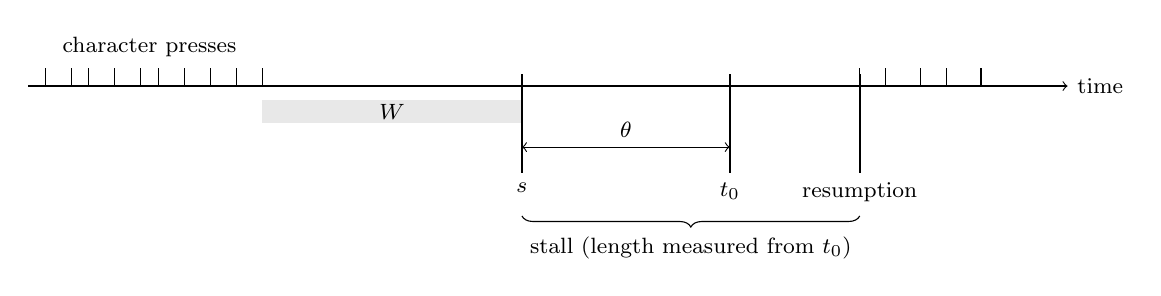
\begin{tikzpicture}[x=0.11cm,y=0.5cm,font=\footnotesize]
  \draw[->] (0,0) -- (120,0) node[right] {time};
  \foreach \x in {2,5,7,10,13,15,18,21,24,27} \draw (\x,0) -- (\x,0.45);
  \foreach \x in {96,99,103,106,110} \draw (\x,0) -- (\x,0.45);
  \node[above] at (14,0.5) {character presses};
  \draw[fill=figband,draw=none] (27,-0.35) rectangle (57,-0.95);
  \node at (42,-0.65) {$W$};
  \draw[thick] (57,0.3) -- (57,-2.2) node[below] {$s$};
  \draw[thick] (81,0.3) -- (81,-2.2) node[below] {$t_0$};
  \draw[<->] (57,-1.55) -- node[above] {$\theta$} (81,-1.55);
  \draw[thick] (96,0.3) -- (96,-2.2) node[below] {resumption};
  \draw[decorate,decoration={brace,mirror,amplitude=4pt}] (57,-3.3) -- node[below=4pt] {stall (length measured
  from $t_0$)} (96,-3.3);
\end{tikzpicture}
\caption{The stall detector. Condition A (fewer than one net character press in the window $W$, shaded) becomes true at
$s$; if it stays true for $\theta$, an onset is raised at $t_0 = s + \theta$. The stall ends at the next character
press.}
\label{fig:detector}
\end{figure}

\subsection{The four axes and the 89 definitions}
\label{sec:grid}

We varied four choices that every such detector has to make, each over levels drawn from prior practice or set around
the default (Table~\ref{tab:grid}). The full crossing gives 90 definitions; with the baseline removed, 89 remain, and
all proportions below are out of 89 and describe this grid, not a sample of possible definitions. The two families of
$\theta$ are different constructs: a quantile of the writer's own intervals marks a pause that is long \emph{for this
writer}, a fixed number of seconds marks a pause that is long in absolute terms. We report them together because both
are in use, and separately where they part (53 definitions with a writer quantile, 36 with fixed seconds).

\begin{table}[t]
\centering\footnotesize
\caption{The four axes of the stall detector. The baseline level is marked with an asterisk. The grid of default and
precedented levels keeps the default window and condition, which have no use outside the detector, and the levels with
precedent outside it: writer-relative thresholds as a kind, the 10-s threshold and the three segmentations (12
definitions, including the baseline). A fixed $\theta$ is a hold after condition A rises, so a 10-s $\theta$ is not the
same construct as a 10-s pause threshold.}
\label{tab:grid}
\begin{tabularx}{\textwidth}{@{}l l X@{}}
\toprule
Axis & Levels & Source of the levels \\
\midrule
Window $W$ & 15, 30$^\ast$, 60~s & 30~s is the default; 15 and 60~s are half and double the default; we found no
use of a window length outside the detector \\
Threshold $\theta$ & writer quantile 0.95, 0.99$^\ast$, 0.995; fixed 10, 30~s & writer-relative thresholds are in use
(an ex-Gaussian bound per writer \cite{chukharev2014pauses}, ten times the within-word median \cite{guo2020scenario}),
though not at these quantiles; fixed thresholds in writing span about 0.25--10~s \cite{torrance2024methods}, so 10~s
has precedent and 30~s, set equal to the default window, has none \\
Condition A & net$^\ast$ (characters $-$ deletions $< 1$); characters only ($< 1$) & whether deletions cancel character
presses; neither rule has a use outside the detector \\
Observation & default intervals$^\ast$; split at key-press gaps of 5~min; of 30~min & 5~min of inactivity as
time-on-task \cite{hart2023time}; 30~min as a session timeout \cite{halfaker2015session} \\
\bottomrule
\end{tabularx}
\end{table}

\paragraph{The pause family.} The second detector counts a pause whenever two consecutive key presses in the same
observation interval are more than a threshold apart. We crossed two kinds of interval (between any two key presses,
or between two character presses), three fixed thresholds (2, 5 and 10~s, within the range used in writing
\cite{torrance2024methods}) and the three segmentations, for 18 definitions. We also computed 18 definitions with the
writer's 0.95, 0.99 and 0.995 quantile over the unit as the threshold; such a threshold labels a fixed share of each
writer's intervals, so its rate is close to that share times the writer's rate of key presses, and we report these as
a control for the key-press rate rather than as pause labels (S3). The pause family is not a check of the stall
results but the same diagnostic applied to a second detector.

\subsection{What we measured}
\label{sec:measures}

\paragraph{Rates and ratios.} The rate is the number of stalls or pauses per observed hour, pooled over a dataset's
units. For each definition we compared the rank order of the four datasets with the baseline order, and the ratio of
the rates of each pair of datasets with the baseline ratio.

\paragraph{The essay-score association.} In KLiCKe, the Spearman correlation of a writer's rate with the
holistic score. Because the sample is large, weak correlations have intervals that exclude zero, so we also describe magnitudes,
using $|\rho| < 0.1$ as negligible and 0.3 as moderate \cite{cohen1988power}.

\paragraph{Adjustments.} Two partial Spearman correlations of score and rate: given typing speed, the median of a
writer's intervals shorter than 2~s, measured six ways (S3); and given the essay's length in characters and the length
of observation. Essay length is part of what raters judge, so the length-adjusted value is the association with the
part of the rate that does not overlap with length, not an effect.

\paragraph{Overdispersion within writers.} For sub-writer units (CS1 work blocks and assignments; CoAuthor sessions),
the Pearson dispersion index $\varphi = \sum (n - \hat e)^2 / \hat e \,/\, (k - p)$, where the expected count $\hat e$ is
the writer's own rate times the unit's exposure and $p$ the number of writers. $\varphi = 1$ is what counting at a
constant rate within a writer would give; we read $\varphi$ as the departure from a constant rate, with 1.5 as a
working threshold, not as a choice between count models, because the window of the detector, dependence between
stalls and the mean structure all affect it (S4).

\paragraph{Components of stall length.} A linear mixed model of log stall length with random effects of writer,
assignment, day and work block (CS1; days are runs of blocks separated by gaps of 6~h or more) or of writer and
session (CoAuthor), fitted by REML; we report the share of each level and of the residual, the stall-to-stall
variation. Stalls that did not resume within their interval are excluded (S5). We do not report the analogous
decomposition of counts, whose estimates did not recover simulated components (S6).

\paragraph{Intervals.} All intervals are 95\% percentile intervals from 2,000 resamples of writers, with each
writer's labels as detected. Two-stage intervals that also redraw the writer-quantile $\theta$ are a
sensitivity analysis (S2). The interval of a
definition shows sampling variation; the spread across definitions shows definitional variation, and we set the two
side by side \cite{robitzsch2022multiverse}. Definitions share axes and are not independent, so we read counts as
proportions of the grid and do not test the grid as a whole \cite{simonsohn2020specification}.

\subsection{Status of the analyses}
\label{sec:status}

Every computation ran under conditions committed in the author's repository before it ran; these are not third-party
registrations. S1 gives the order of the computations, including those added after seeing results,
and the status of each conclusion. The speed covariate was chosen twice after seeing results, so the speed-adjusted values are exploratory. Three points bear
on the claims. The criterion for a reversal of a rate ratio (25\% of the
definitions for a pair) was set after the number of reversed point values per pair had been seen, and the pair committed
to be reported first, the two CS1 editions, did not reach it. The criterion for a reversal of the score association
required only one definition with an interval on the other side of zero, which is lenient, so we report the full
distribution; requiring the point value to lie there as well, a rule added later, changed no count. Sizes, the
reading by classes of interval and the grid of default and precedented levels were set after seeing the results.

The author used Claude (Anthropic) to search the literature, to write the analysis scripts under these conditions and
to check the numbers in the text against the result files; every number in the text was compared with the result files.

\section{Results}
\label{sec:results}

\subsection{The label--essay-score association moves with the definition, in direction only at some levels}
\label{sec:res-score}

A study that reports how a pause or stall rate relates to the quality of a product usually reports one definition. We
asked whether that association depends on the definition, and measured, for each definition, the Spearman
correlation between the KLiCKe writers' rates and their holistic scores, with a resampled interval
(Figure~\ref{fig:score}, Table~\ref{tab:pause}).

\paragraph{Stalls.} Under the baseline the correlation was $-0.063$ [$-0.091$, $-0.034$]. Two criteria had been set
before the association was seen. The presence of an association would count as moving if the share of definitions
with an interval excluding zero lay between 25\% and 75\%; it was 82 of 89 (92\%), so by that criterion presence did not
move. The direction would count as changing if one definition had an interval on the other side of zero; 10 did (also
when the point value is required to lie there), so the direction changed. All 10 had the shortest window,
$W = 15$~s, the level we set at half the default, and a writer-quantile $\theta$; among the 59 definitions with
other windows, 57 were negative and none was positive, and on the grid of default and precedented levels
(Table~\ref{tab:grid}) none was positive either. Across the 89 definitions the
correlation ranged from $-0.25$ to $+0.14$ (median $-0.14$), with intervals negative for 72, positive for 10 and
including zero for 7. By point value, 58 definitions gave a negative correlation of at least 0.1 in absolute value and 3
a positive one; all 36 fixed-second definitions were negative. The positive corner is not a floor effect of rare
stalls (S3).

\paragraph{Pauses.} For the second detector the reading set in advance was that the direction changes if at least one
definition has an interval above zero and one below. With fixed thresholds, the interval was below zero for 7 of the 18
definitions, all but one at 10~s, and above zero for 3, on character intervals at 2 and 5~s (Table~\ref{tab:pause}).
The direction therefore changed, but between mostly negligible values: 13 of the 18 intervals lay within $\pm 0.1$, and only two definitions at
10~s had a point value at or below $-0.10$ ($-0.101$ and $-0.127$). By the criterion for presence used for stalls, which was not
set in advance for pauses, 10 of 18 intervals (56\%) excluded zero, so presence moved as well. The 10-s values are
smaller in magnitude than the $-0.15$ to $-0.43$ reported for pause durations and latencies, a different measure
(Section~\ref{sec:related}). The 18 definitions with a writer-quantile threshold, a control for the rate of key presses
(Section~\ref{sec:grid}), correlated with the score at $+0.58$ to $+0.67$, close to the 0.62 of the rate of key presses
itself; the reading stated for all 36 definitions is in S1.

A reader who took one definition would report a small negative relation (any fixed stall threshold), a
negligible one (the stall baseline, most fixed pause thresholds), or a positive one (a 15-s stall window with a writer
quantile); a writer-quantile pause threshold would report the rate of key presses.

\begin{figure}[t]
\centering
\begin{tikzpicture}
\begin{axis}[name=raw, width=\textwidth, height=4.8cm, xmin=0, xmax=91, ymin=-0.33, ymax=0.28,
  ylabel={Spearman $\rho$}, xticklabels={}, ytick={-0.3,-0.2,-0.1,0,0.1,0.2}, grid=major, grid style={figband},
  title={(a) Stall rate and holistic score, 90 definitions ordered by $\rho$}, title style={font=\footnotesize},
  tick label style={font=\footnotesize}, label style={font=\footnotesize},
  legend style={font=\scriptsize, at={(0.02,0.98)}, anchor=north west}, legend cell align=left]
  \addplot[only marks, mark=*, mark size=1.1pt, color=figc1, error bars/.cd, y dir=both, y explicit,
    error bar style={color=figc1!60}] table[x=i, y=rho, y error plus expr=\thisrow{hi}-\thisrow{rho},
    y error minus expr=\thisrow{rho}-\thisrow{lo}, discard if not={fam}{1}] {figdata/score.csv};
  \addlegendentry{writer-quantile $\theta$}
  \addplot[only marks, mark=square*, mark size=1.1pt, color=figc2, error bars/.cd, y dir=both, y explicit,
    error bar style={color=figc2!60}] table[x=i, y=rho, y error plus expr=\thisrow{hi}-\thisrow{rho},
    y error minus expr=\thisrow{rho}-\thisrow{lo}, discard if not={fam}{0}] {figdata/score.csv};
  \addlegendentry{fixed-second $\theta$}
  \addplot[only marks, mark=star, mark size=3.5pt, thick, color=black] table[x=i, y=rho, discard if not={b0}{1}]
    {figdata/score.csv};
  \addlegendentry{baseline}
  \addplot[only marks, mark=triangle, mark size=2.2pt, color=black] table[x=i, y expr=\thisrow{hi}+0.03,
    discard if not={W15}{1}] {figdata/score.csv};
  \addlegendentry{$W = 15$~s}
  \draw[black, thin] (axis cs:0,0) -- (axis cs:91,0);
\end{axis}
\begin{axis}[name=spd, at={(raw.south)}, anchor=north, yshift=-0.9cm, width=\textwidth, height=4cm, xmin=0, xmax=91,
  ymin=-0.33, ymax=0.2, ylabel={partial $\rho$}, xticklabels={}, ytick={-0.3,-0.2,-0.1,0,0.1}, grid=major,
  grid style={figband}, title={(b) Given typing speed (median interval $< 2$~s; exploratory)},
  title style={font=\footnotesize}, tick label style={font=\footnotesize}, label style={font=\footnotesize}]
  \addplot[only marks, mark=*, mark size=1.1pt, color=figc1, error bars/.cd, y dir=both, y explicit,
    error bar style={color=figc1!60}] table[x=i, y=adj, y error plus expr=\thisrow{ahi}-\thisrow{adj},
    y error minus expr=\thisrow{adj}-\thisrow{alo}, discard if not={fam}{1}] {figdata/score.csv};
  \addplot[only marks, mark=square*, mark size=1.1pt, color=figc2, error bars/.cd, y dir=both, y explicit,
    error bar style={color=figc2!60}] table[x=i, y=adj, y error plus expr=\thisrow{ahi}-\thisrow{adj},
    y error minus expr=\thisrow{adj}-\thisrow{alo}, discard if not={fam}{0}] {figdata/score.csv};
  \addplot[only marks, mark=star, mark size=3.5pt, thick, color=black] table[x=i, y=adj, discard if not={b0}{1}]
    {figdata/score.csv};
  \draw[black, thin] (axis cs:0,0) -- (axis cs:91,0);
\end{axis}
\begin{axis}[at={(spd.south)}, anchor=north, yshift=-0.9cm, width=\textwidth, height=4cm, xmin=0, xmax=91,
  ymin=-0.33, ymax=0.2, ylabel={partial $\rho$}, xlabel={definitions (same order as panel a)}, xticklabels={},
  ytick={-0.3,-0.2,-0.1,0,0.1}, grid=major, grid style={figband},
  title={(c) Given essay length and length of observation}, title style={font=\footnotesize},
  tick label style={font=\footnotesize}, label style={font=\footnotesize}]
  \addplot[only marks, mark=*, mark size=1.1pt, color=figc1, error bars/.cd, y dir=both, y explicit,
    error bar style={color=figc1!60}] table[x=i, y=ln, y error plus expr=\thisrow{lhi}-\thisrow{ln},
    y error minus expr=\thisrow{ln}-\thisrow{llo}, discard if not={fam}{1}] {figdata/score.csv};
  \addplot[only marks, mark=square*, mark size=1.1pt, color=figc2, error bars/.cd, y dir=both, y explicit,
    error bar style={color=figc2!60}] table[x=i, y=ln, y error plus expr=\thisrow{lhi}-\thisrow{ln},
    y error minus expr=\thisrow{ln}-\thisrow{llo}, discard if not={fam}{0}] {figdata/score.csv};
  \addplot[only marks, mark=star, mark size=3.5pt, thick, color=black] table[x=i, y=ln, discard if not={b0}{1}]
    {figdata/score.csv};
  \draw[black, thin] (axis cs:0,0) -- (axis cs:91,0);
\end{axis}
\end{tikzpicture}
\caption{The stall--score association in KLiCKe (4,908 writers) for the baseline and the 89 definitions, with 95\%
intervals from resampling writers. Triangles mark the definitions with $W = 15$~s. Panels (b) and (c) keep the order of panel (a).}
\label{fig:score}
\end{figure}

\begin{table}[t]
\centering\footnotesize
\caption{The pause family: the association of the pause rate with the holistic score in KLiCKe, range over the three
segmentations for each kind of interval and threshold, and the number of the three with an interval below or above
zero. Every definition is in S3.}
\label{tab:pause}
\begin{tabular}{@{}l l r r r@{}}
\toprule
Interval & Threshold & $\rho$ & Below zero & Above zero \\
\midrule
any key & 2~s & $-0.01$ to $+0.03$ & 0 & 0 \\
 & 5~s & $-0.04$ to $0.00$ & 1 & 0 \\
 & 10~s & $-0.13$ to $-0.09$ & 3 & 0 \\
character & 2~s & $+0.01$ to $+0.05$ & 0 & 2 \\
 & 5~s & $0.00$ to $+0.03$ & 0 & 1 \\
 & 10~s & $-0.10$ to $-0.06$ & 3 & 0 \\
any key & quantile 0.95--0.995 & $+0.58$ to $+0.62$ & 0 & 9 \\
character & quantile 0.95--0.995 & $+0.62$ to $+0.67$ & 0 & 9 \\
\bottomrule
\end{tabular}
\end{table}

\subsection{Adjusting for essay length leaves no stall definition negative and most values negligible}
\label{sec:res-adjust}

Two quantities that do not contain the labels can carry the association: how much a writer writes and how fast.
Essay length correlated with the score at 0.75 [0.73, 0.76], and faster writers had higher scores (Spearman $-0.53$
between the score and the median short interval, a lower interval meaning faster typing). The length of observation
barely varied in KLiCKe (interquartile range 26--29~min) and correlated with the score at 0.10.

\paragraph{Given essay length.} Given essay length and the length of observation, the partial correlation of score and
stall rate was positive with an interval above zero for 54 definitions, included zero for 35 and was below zero for
none ($+0.02$ to $+0.13$; baseline $+0.057$ [$+0.029$, $+0.085$]); the 10 definitions that were positive without
adjustment stayed positive. By the reading set before the computation, the sign became uniform: no definition was
negative. In size, 74 of the 89 intervals lay within $\pm 0.1$, so after adjustment the stall rate carried little
association with the score. Stalls and essay length overlap by construction: under the net rule a stall is a period in
which the text does not grow, so the adjustment also removes part of what the stall rate measures. For the fixed pause
thresholds, 15 of 18 were positive and none negative, and 9 had an interval above $+0.1$.

\paragraph{Given typing speed (exploratory).} With the median of intervals under 2~s, the partial correlation of score and stall rate was
negative with an interval below zero for all 89 definitions ($-0.29$ to $-0.03$; baseline $-0.18$ [$-0.21$, $-0.15$]),
and below $-0.1$ for 71; the ten definitions with a positive unadjusted interval all had an interval below zero.
Six ways of measuring speed gave no positive interval and 2 of
534 intervals including zero (S3). For the fixed pause thresholds the speed-adjusted correlation went
the other way: positive for 11 of 18 and negative for 4.

Neither adjusted value is a causal effect (Section~\ref{sec:discussion}).

\paragraph{Reading by classes of interval.} Table~\ref{tab:read} applies the reading proposed in
Section~\ref{sec:discussion}, formed after seeing these results.
Unadjusted, the fixed stall thresholds read as below $-0.1$ and the fixed pause thresholds as negligible, while the full
stall grid depended on the definition. On the grid of default and precedented levels the reading split by the family of
$\theta$, which the grid treats as two constructs (Section~\ref{sec:grid}): the fixed 10-s threshold read as below
$-0.1$ and the writer quantile as negligible, each consistently. Given length, every stall group read as negligible, but
the fixed pause thresholds came to depend on the definition, with 9 of 18 above $+0.1$: adjustment changed the reading
as a definition does. Given speed, the full grid fell just short of a consistent reading (89.9\%).

\begin{table}[t]
\centering\scriptsize\setlength{\tabcolsep}{3pt}
\caption{Reading of the score association by classes of interval (a rule proposed after seeing the results). Each
cell gives the reading, the share of the leading class among the classified definitions, and the counts below
$-0.1$ / within $\pm 0.1$ / above $+0.1$ / imprecise. Groups with the baseline: the default and precedented grid and
its writer-quantile part; the full grid excludes it.}
\label{tab:read}
\begin{tabular}{@{}l l l l@{}}
\toprule
Group (definitions) & Unadjusted & Given length & Given speed (exploratory) \\
\midrule
Stalls, full grid (89) & depends (71\%): 48/17/2/22 & negligible (98\%): 0/74/1/14 & depends (89.9\%): 71/8/0/10 \\
Stalls, fixed $\theta$ (36) & below (100\%): 36/0/0/0 & negligible (100\%): 0/33/0/3 & below (100\%): 36/0/0/0 \\
Stalls, writer quantile (53) & depends (54\%): 12/17/2/22 & negligible (97\%): 0/41/1/11 & depends (81\%): 35/8/0/10 \\
Stalls, default and precedented (12) & depends (62\%): 3/5/0/4 & negligible (100\%): 0/9/0/3 & below (100\%): 12/0/0/0 \\
\quad of which fixed 10~s (3) & below (100\%): 3/0/0/0 & negligible (100\%): 0/3/0/0 & below (100\%): 3/0/0/0 \\
\quad of which writer quantile (9) & negligible (100\%): 0/5/0/4 & negligible (100\%): 0/6/0/3 & below (100\%): 9/0/0/0 \\
Pauses, fixed threshold (18) & negligible (100\%): 0/13/0/5 & depends (60\%): 0/6/9/3 & depends (81\%): 0/9/2/7 \\
\bottomrule
\end{tabular}
\end{table}

\subsection{The same diagnostic applied to other conclusions}
\label{sec:res-other}

The diagnostic applies to any conclusion drawn from the labels. We applied it to three more: a comparison of rates
between datasets, a count model within writers, and the decomposition of stall length.

\paragraph{Comparing rates between datasets.}
\label{sec:res-ratio}
Does a comparison of stall rates between datasets, such as between cohorts of a course, survive a change of
definition? Under the baseline the rates were
15.1 (KLiCKe), 13.1 (CS1 2019), 8.8 (CS1 2021) and 7.1 (CoAuthor) per hour; across the 89 definitions, the CS1 2019
rate alone ranged from 4.4 to 46.0. By the criterion set before the computations (25\% of definitions), the rank
order of the four datasets moved: it differed from the baseline order for 80 of 89 definitions, although the close
baseline rates of CS1 2019 and KLiCKe swap alone in 11 of them. We counted a ratio as reversed when its point value and its
interval lay on the other side of 1 from the baseline ratio, a description of each definition rather than a test over
the grid (Figure~\ref{fig:ratio}). For the two CS1 editions,
which share the course and the recording and which we had committed to report first, 20 of 89 definitions (22\%)
reversed the ratio, below the 25\% we had set after seeing point values (Section~\ref{sec:status}; 22 of 89 in
the time after the 100th interval, S2), but 23 (26\%), above it, when the first 60~s of each observation interval
were also excluded (S2); 18 of the 20 used a fixed $\theta$. Every fixed-$\theta$ definition reversed both comparisons of
CS1 with KLiCKe (66 and 53 reversals in all); CS1 2019 against CoAuthor reversed for 6 and the two
writing datasets for none (S3). Among the
fixed pause thresholds, the two CS1 editions reversed for none of 18, whereas the pairs with CoAuthor, whose pause rates
ranged from 42 to 498 per hour, reversed for 14 and 13 (S3), so by the same criterion the direction of a ratio changed in the pause family too. The
counts are not comparable across pairs, whose
baseline ratios and sample sizes differ.

\begin{figure}[t]
\centering
\begin{tikzpicture}
\begin{axis}[name=a, width=0.52\textwidth, height=5cm, xmin=0, xmax=91, ymin=-1.1, ymax=1.2, xticklabels={},
  ylabel={log rate ratio}, xlabel={definitions ordered by ratio}, grid=major, grid style={figband},
  title={(a) CS1 2019 / CS1 2021}, title style={font=\footnotesize}, tick label style={font=\footnotesize},
  label style={font=\footnotesize}]
  \addplot[only marks, mark=*, mark size=1pt, color=figc1, error bars/.cd, y dir=both, y explicit,
    error bar style={color=figc1!60}] table[x=i, y=lr, y error plus expr=\thisrow{hi}-\thisrow{lr},
    y error minus expr=\thisrow{lr}-\thisrow{lo}, discard if not={fam}{1}] {figdata/ratio_cs19_cs21.csv};
  \addplot[only marks, mark=square*, mark size=1pt, color=figc2, error bars/.cd, y dir=both, y explicit,
    error bar style={color=figc2!60}] table[x=i, y=lr, y error plus expr=\thisrow{hi}-\thisrow{lr},
    y error minus expr=\thisrow{lr}-\thisrow{lo}, discard if not={fam}{0}] {figdata/ratio_cs19_cs21.csv};
  \addplot[only marks, mark=star, mark size=3.5pt, thick, color=black] table[x=i, y=lr, discard if not={b0}{1}]
    {figdata/ratio_cs19_cs21.csv};
  \draw[black, thin] (axis cs:0,0) -- (axis cs:91,0);
\end{axis}
\begin{axis}[at={(a.east)}, anchor=west, xshift=0.9cm, width=0.52\textwidth, height=5cm, xmin=0, xmax=91,
  ymin=-1.1, ymax=1.2, xticklabels={}, xlabel={definitions ordered by ratio}, grid=major, grid style={figband},
  title={(b) CS1 2019 / KLiCKe}, title style={font=\footnotesize}, tick label style={font=\footnotesize},
  label style={font=\footnotesize}]
  \addplot[only marks, mark=*, mark size=1pt, color=figc1, error bars/.cd, y dir=both, y explicit,
    error bar style={color=figc1!60}] table[x=i, y=lr, y error plus expr=\thisrow{hi}-\thisrow{lr},
    y error minus expr=\thisrow{lr}-\thisrow{lo}, discard if not={fam}{1}] {figdata/ratio_cs19_kl.csv};
  \addplot[only marks, mark=square*, mark size=1pt, color=figc2, error bars/.cd, y dir=both, y explicit,
    error bar style={color=figc2!60}] table[x=i, y=lr, y error plus expr=\thisrow{hi}-\thisrow{lr},
    y error minus expr=\thisrow{lr}-\thisrow{lo}, discard if not={fam}{0}] {figdata/ratio_cs19_kl.csv};
  \addplot[only marks, mark=star, mark size=3.5pt, thick, color=black] table[x=i, y=lr, discard if not={b0}{1}]
    {figdata/ratio_cs19_kl.csv};
  \draw[black, thin] (axis cs:0,0) -- (axis cs:91,0);
\end{axis}
\end{tikzpicture}
\caption{Log ratios of stall rates with 95\% intervals. Circles: writer-quantile $\theta$; squares: fixed seconds;
star: baseline. A ratio reverses when its point value and its interval lie on the other side of zero from the baseline.}
\label{fig:ratio}
\end{figure}

\paragraph{Departure from a constant rate within writers.}
\label{sec:res-phi}
Do the counts of a writer's sub-units vary more than a constant rate per writer would make them vary? The answer
decides how much dispersion a count model of stalls has to allow. We measured the dispersion index $\varphi$ with the writer's own rate as the expectation (Table~\ref{tab:phi},
Figure~\ref{fig:phi}). Under the baseline, $\varphi$ exceeded 1 in all four CS1 cells (1.44 to 3.82) and not in
CoAuthor sessions (1.08). Across the 89 definitions, the median $\varphi$ was close to 1 in CS1 2019 blocks and CoAuthor
sessions (1.03 and 1.02), 1.21 in CS1 2021 blocks and 1.25 and 2.28 in the CS1 assignments; the interval exceeded 1 for
43 to 68 definitions in the CS1 cells and for 7 in CoAuthor. The baseline lay above the median of the 89 definitions in
every CS1 cell. The conclusion against 1.5 reversed, by the same counting rule, for 54 definitions in the CS1 2019
assignments, 49 in the CS1 2021 blocks, 19 (21\%) in the CS1 2021 assignments and none in CoAuthor; in CS1 2019 blocks
the baseline interval contained 1.5, so no reversal was counted. In the
CS1 2019 assignments and the CS1 2021 blocks, then, whether $\varphi$ lay above or below 1.5 depended on the definition;
in the other cells the reversals stayed under 25\% or could not be counted. Restricted to the time after the 100th
interval, the two cells were the CS1 2019 and CS1 2021 assignments (57 and 26 reversals), because the CS1 2021 blocks
could no longer be counted, and so they were when the first 60~s of each observation interval were also excluded
(57 and 24; S2). $\varphi$ compares variance with the mean
and does not show which assumption of a count model fails.

\begin{table}[t]
\centering\footnotesize
\caption{Dispersion index $\varphi$ within writers. Baseline with 95\% interval; median and range over the 89
definitions; number of definitions whose interval exceeds 1; number whose point value and interval lie on the other
side of 1.5 from the baseline (--: the baseline interval contains 1.5).}
\label{tab:phi}
\begin{tabular}{@{}l l r r r r@{}}
\toprule
Cell & Baseline & Median & Range & Interval $> 1$ & Reversed at 1.5 \\
\midrule
CS1 2019 blocks & 1.44 [1.35, 1.52] & 1.03 & 0.67--3.28 & 43 & -- \\
CS1 2019 assignments & 1.95 [1.75, 2.15] & 1.25 & 0.74--3.72 & 57 & 54 \\
CS1 2021 blocks & 1.82 [1.58, 2.11] & 1.21 & 0.56--4.66 & 46 & 49 \\
CS1 2021 assignments & 3.82 [3.13, 4.56] & 2.28 & 0.63--7.87 & 68 & 19 \\
CoAuthor sessions & 1.08 [0.98, 1.19] & 1.02 & 0.80--1.37 & 7 & 0 \\
\bottomrule
\end{tabular}
\end{table}

\begin{figure}[t]
\centering
\begin{tikzpicture}
\begin{axis}[width=\textwidth, height=5cm, xmin=0, xmax=461, ymin=0.4, ymax=8.2, ymode=log, log basis y=10,
  ytick={0.5,1,1.5,2,4,8}, yticklabels={0.5,1,1.5,2,4,8}, ylabel={$\varphi$}, xtick={45,137,229,321,413},
  xticklabels={CS1 2019 blocks, CS1 2019 assign., CS1 2021 blocks, CS1 2021 assign., CoAuthor sessions},
  tick label style={font=\scriptsize}, label style={font=\footnotesize}, grid=major, grid style={figband}]
  \addplot[only marks, mark=*, mark size=0.8pt, color=figc1, error bars/.cd, y dir=both, y explicit,
    error bar style={color=figc1!50}] table[x expr=(\thisrow{cell}-1)*92+\thisrow{i}, y=phi,
    y error plus expr=\thisrow{hi}-\thisrow{phi}, y error minus expr=\thisrow{phi}-\thisrow{lo}] {figdata/phi.csv};
  \addplot[only marks, mark=star, mark size=3.5pt, thick, color=black] table[x expr=(\thisrow{cell}-1)*92+\thisrow{i},
    y=phi, discard if not={b0}{1}] {figdata/phi.csv};
  \draw[black, thin] (axis cs:0,1) -- (axis cs:461,1);
  \draw[black, dashed] (axis cs:0,1.5) -- (axis cs:461,1.5);
\end{axis}
\end{tikzpicture}
\caption{The dispersion index within writers for the 90 definitions in each cell, ordered by value, with 95\%
intervals; star: baseline. Solid line: 1 (constant rate within a writer); dashed line: 1.5.}
\label{fig:phi}
\end{figure}

\paragraph{Components of stall length.}
\label{sec:res-length}
A map of what moves needs a side that stays. Is the decomposition of stall length as fragile as the rates? We fitted
the decomposition for all 90 definitions (Figure~\ref{fig:length}). The lengths are times from onset to resumption, so
a change of definition changes both the stalls and the point from which they are measured. Under the baseline, the stall-to-stall share was
0.93 (CS1 2019) and 0.92 (CS1 2021), and the writer share 0.03 in both, which can be read as the intraclass correlation
of writers. In both CS1 editions, the stall-to-stall share stayed the largest component in every one of the 89
definitions (0.88 to 1.00), at least 0.83 above the next component, and the writer share stayed small (0.00 to 0.05);
we did not compute intervals for these shares. The excluded unresumed stalls were 0.5--7\% of the CS1
stalls, depending on the definition. CoAuthor kept the same order in 86 of 89 definitions (S5). This is a weak contrast: most variance sitting at the lowest level is common for event-level
outcomes (S5).

\begin{figure}[t]
\centering
\begin{tikzpicture}
\begin{axis}[width=\textwidth, height=4.6cm, xmin=0, xmax=277, ymin=0, ymax=1.05, ylabel={share of variance},
  xtick={45,137,229}, xticklabels={CS1 2019, CS1 2021, CoAuthor}, tick label style={font=\footnotesize},
  label style={font=\footnotesize}, grid=major, grid style={figband},
  legend style={font=\scriptsize, at={(0.5,0.55)}, anchor=center}, legend cell align=left]
  \addplot[only marks, mark=*, mark size=0.9pt, color=figc1] table[x expr=(\thisrow{ds}-1)*92+\thisrow{i},
    y=stall] {figdata/lengths.csv};
  \addlegendentry{stall to stall}
  \addplot[only marks, mark=square*, mark size=0.9pt, color=figc2] table[x expr=(\thisrow{ds}-1)*92+\thisrow{i},
    y=writer] {figdata/lengths.csv};
  \addlegendentry{writer}
\end{axis}
\end{tikzpicture}
\caption{Shares of the variance of log stall length for the 90 definitions in each dataset, each series ordered by
value. The remaining shares (assignment, day, block or session) are in S5.}
\label{fig:length}
\end{figure}

\section{Discussion}
\label{sec:discussion}

The stall--score association changed direction only where a 15-s window met a writer quantile, the pause association
changed between mostly negligible values, and adjusting for length moved both upwards. For researchers in educational
data mining and learning analytics who relate pause, stall or inactivity rates to outcomes or compare them across
datasets, a report should therefore contain the range of the
conclusion across definitions and adjustments, with intervals, rather than the point value of one definition. On the
default and precedented stall levels, our result resembles earlier multiverse analyses, in which an eye-movement effect
kept its existence and changed its size \cite{godwin2025multiverse} and boundary pausing in CS1 changed strength with
the split at 2~s but not direction \cite{koutcheme2026keystroke}; widening the grid to levels around the default also
changed the direction.

\paragraph{Why the direction can change.} A rate of labels per hour is a count, and counts carry how much and how fast
a writer types as well as how often the writer stops. A writer-quantile pause threshold makes this explicit: its rate
follows the rate of key presses and correlated with the score at about $+0.6$. Prior work reports the same split
between counts and durations: pause counts can correlate positively with scores through text length, whereas pause
durations correlate negatively \cite{schaller2026keyscore}. Given length both detectors moved upwards, but
given speed, an exploratory analysis, they answered differently: every stall definition was negative while most fixed
pause thresholds were positive. The ten positive stall definitions, which pair a short window with a writer quantile,
all turned negative given speed, so that corner may follow typing speed through the writer quantile. These are
patterns, not a tested mechanism; the association that remains after either adjustment is the part of the rate that
does not overlap with the covariate, and speed and length may confound or mediate it \cite{mackinnon2000equivalence}.

\paragraph{Existing answers to arbitrary thresholds.} Mixture models, personalised thresholds, state models, location
classes and controls for typing skill (Section~\ref{sec:related}) each choose a threshold, a model or a control. The
diagnostic applies to them in the same way: vary the choice they make and report whether the conclusion moves. Methods
that keep the uncertainty of the choice, such as probabilistic assignment of pauses to components or averaging over
models, are the natural complement.

\paragraph{What the criteria established.} The changes of direction (by a lenient criterion), the stable presence of
the stall association, the moving rank order, the length-adjusted stall values, $\varphi$ against 1.5 and the stable
length component rest on criteria set before each quantity was seen; the rest was judged after seeing results or is
exploratory (S1). We did not test whether the definitional spread changes the performance of a predictor
or a decision about when to intervene.

\paragraph{Recommendation.} When reporting an association or a comparison based on a pause or stall rate, report the
value of each axis, vary each axis over its range in prior practice and around the default, and report the spread with
intervals, with and without adjustment for quantities that do not contain the label, such as the length of the
product; adjustment is an axis as well, since it can change the conclusion as a definition can. As a proposal formed
after seeing these results, sort each definition's interval into below $-0.1$, above $+0.1$, within $\pm 0.1$
(negligible) or imprecise (crossing a bound). Read a group as imprecise when at least half of its intervals are, as a
consistent direction or a negligible association when one class holds at least 90\% of the classified definitions, and
otherwise as dependent on the definition, a reading that includes moves between negative and negligible values; give
the share of the leading class and the number of imprecise intervals with each reading, since the reading is sensitive
near the 90\% bound. Because these shares depend on how finely each axis is cut and on which constructs are pooled,
apply the reading to the grid of the default and of levels with precedent, within each family of thresholds, and to the
grid with the levels around the default added (Table~\ref{tab:read}). The band of $\pm 0.1$ is for correlations;
ratios and $\varphi$ need their own reference points and bands. The code is released for this purpose.

\section{Limitations}
\label{sec:limitations}

\paragraph{No ground truth.} The data have no self-reports or think-aloud, so we cannot say which definition is right.
A stall is a stop in net character production, not a judgement that the writer was stuck.

\paragraph{The range varied.} All proportions are of the definitions examined. The stall grid is centred on one
detector's default, no window length has a use outside the detector, and fixed thresholds make up four in ten stall definitions. The
stall detector does not reach pauses shorter than about 15~s, and the pause family covers 2 to 10~s and writer
quantiles; we did not vary thresholds below 2~s, thresholds proportional to within-word speed \cite{guo2020scenario}
or pauses split by linguistic location, because we fixed grids that apply alike to code and essays. We varied the rate per observed hour only; rates per key press or per
word and measures of pause duration, such as mixture components, were not varied, so the recommendation is limited to
rates. We did not compare groups within a dataset.

\paragraph{Differences between datasets.} The datasets differ at once in the task, the recording (CS1 key presses are
reconstructed from edit events) and the length of units, so differences between them are not attributed to a cause.

\paragraph{Intervals and samples.} The primary intervals hold each writer's quantile threshold as detected and leave
out its variation. A resample that redraws it causally left the score and ratio conclusions as they were, but for
$\varphi$ it was shifted above the point values, so how the variation of the threshold bears on $\varphi$ is not
resolved (S2). The default observation intervals depend on the companion study's estimator; every result is also
reported for two segmentations that need only the time of each key press and whether it inserted or deleted a
character.
A definition changes the time in which a stall can be detected (the writer-quantile family
cannot detect before the 100th interval, 3.2--10.3\% of the exposure), which units reach 5 minutes of exposure and, for $\varphi$, which writers
have stalls at all, so definitions differ in their samples as well as their labels. Removing the undetectable time (Section~\ref{sec:detector})
changed no score interval from one side of zero to the other, but moved the CS1 ratio and $\varphi$ in the CS1 2021
assignments above 25\% and left the CS1 2021 blocks uncounted (S2).

\paragraph{Counts and lengths.} The levels of variation in counts could not be separated (S6). The dispersion of
assignments includes differences between assignments, and a $\varphi$ near 1 does not establish a Poisson process: the
window of the detector can make counts underdispersed while heterogeneity makes them overdispersed. The length
decomposition excludes stalls that did not resume, and CS1 days are inferred from gaps of 6~h.

\paragraph{One outcome and its length.} The score association rests on one holistic score in KLiCKe and was not checked
against a second outcome. Its inter-rater agreement ($\kappa$ 0.60 before and 0.76 after discussion) is imperfect, which shrinks
correlations towards zero and can move intervals into the negligible class. The score reflects essay length strongly (0.75), so part of any label's association with it
can run through length; and because the observation time is nearly fixed in KLiCKe, time spent in stalls reduces the
time left for writing, so adjusting for length removes part of what the label counts. Speed and length were adjusted linearly on ranks, and non-linear remainders were not examined.
We did not separate stalls by their position in the session (planning early, review or waiting late under the
fixed 30-minute timer), so the positive corner and the positive length-adjusted values cannot be told apart from that
route. The score association rests on adults recruited online, not on a course. We did not evaluate the labels as
predictors. We say nothing about Japanese input, input method editors, natural work
or other populations.

\section{Conclusion}
\label{sec:conclusion}

Across 89 definitions of a window-based stall label and 18 of a fixed-threshold pause label, the association between
the label rate and essay score moved with the definition. For stalls its presence stayed and its direction changed only
where a 15-s window met a writer quantile; on the default and precedented levels the reading split by the family of
threshold. For pauses the direction changed between mostly negligible values. Adjusting for essay length moved both
upwards, leaving no stall definition negative and raising half of the pause definitions above $+0.1$. The rank order of
the datasets moved, a rate ratio between two editions of a programming course reversed for a fifth of the definitions,
below a criterion set after seeing point values but above it when the first minute of each observation interval was
excluded, whether within-writer dispersion exceeded 1.5 depended on the
definition in two CS1 cells, and the largest component of CS1 stall length stayed. In this sample, then, a study that
relates a pause or stall rate to an outcome, or compares rates between datasets, could not rest on one definition or
one adjustment: it should report the range of its conclusion across both, with intervals, and say whether that range
reads as consistent, negligible, dependent on the definition or imprecise.

\section*{Data and code availability}
\label{sec:availability}

No new data were collected; the analyses used de-identified datasets released for research, under the terms set by their authors. The
archive (\url{https://doi.org/10.5281/zenodo.24047695}) holds the detector, the scripts of every computation, the conditions
committed before each computation and the aggregate results by definition. The writers excluded as holdouts are
identified by their public identifiers for KLiCKe and CoAuthor; for CS1, whose files are released by their authors on
request and for which we agreed to publish only aggregate values, the archive gives the rule and the seed that draw
the holdout instead of the identifiers.

\section*{Declaration of Generative AI Software tools in the writing process}

% The wording below follows the journal's required sentence.
During the preparation of this work, the author used Claude (Anthropic) in all sections and in the supplementary
material in order to draft the text, the tables and the figures from the author's analysis records, to write the
analysis scripts under conditions fixed in advance, to search the literature, and to check the numbers against the
result files. After using this tool, the author reviewed and edited the content as needed and takes full
responsibility for the content of the publication.


\bibliographystyle{acmtrans}
\bibliography{references}

\appendix
% Supplementary material, placed after the references as the journal's instructions ask. Sections S1 to S8 are referred
% to from the main text by their numbers.
\renewcommand{\thesection}{S\arabic{section}}
\setcounter{section}{0}

\section{Conditions, status of the analyses and changes}
\label{app:status}

\paragraph{Order of the computations.} Every computation ran under a written condition committed to the author's version
control before it ran. The conditions are in the archive, in Japanese, with an English summary. They are records in
the author's repository, not third-party registrations: their order is shown by the repository, not by an independent
time stamp.

\begin{center}\footnotesize
\begin{tabularx}{\textwidth}{@{}c l X@{}}
\toprule
Order & Status & Computation and what was fixed before it \\
\midrule
1 & [P] & Primary: the 90 definitions, rates, ranks, $\varphi$, agreement in time, the decomposition of counts and lengths
for 9 definitions, an estimator-level comparison (in the archive); the criteria for ``moves'' (25\% of definitions) and for
overdispersion \\
2 & [A] & Length decomposition for all 90 definitions; the criterion that the stall-to-stall share stays the largest \\
3 & [A] & Intervals for rates, ratios and $\varphi$; the KLiCKe score association; the criterion for a reversal of
the score association (one definition with an interval on the other side of zero) and, set after the reversed point
values had been seen and before the intervals, for a ratio (25\% of definitions for a pair) \\
4 & [E] & Partial association given the key-press rate (withdrawn as a covariate, below) \\
5 & [E] & Partial association given typing speed (median interval $< 2$~s) \\
6 & [E] & Six ways of measuring speed and the within-prompt adjustment; the reading sentence stated in
Section~\ref{sec:res-adjust} \\
7 & [A] & After a first internal pre-submission check: the pause family (36 definitions), intervals with the writer
quantile estimated again, and the adjustment for essay and observation length; the readings of each, including that
the two-stage intervals replace the earlier ones regardless of which is narrower \\
8 & [A] & The restriction of all 90 definitions to the time after each unit's 100th interval (S2); its readings \\
9 & [A] & After a second internal check: two-stage intervals with the writer quantile estimated causally (S2), the
counting rule that a reversal needs both the point value and the interval on the other side, and the reading that the
new intervals replace the one-stage ones only if at most 5\% of point values fall outside their intervals; 27\% of
the $\varphi$ values did, so the primary intervals returned to the one-stage ones (the score association,
positive for 10 definitions under the one-stage intervals, had been positive for 14 under those of order 7) \\
10 & [D] & After a third internal check, no new computation: the reading by classes of interval, with imprecise intervals
as a class of their own, and the grid of default and precedented levels, counted from the existing intervals (in the
archive) \\
11 & [A] & After a fourth internal check: the share of exposure in the first $W$ seconds of each observation interval,
and all 90 definitions with each interval cut to start 60~s after its start and not before the 100th interval (S2);
its readings \\
\bottomrule
\end{tabularx}
\end{center}

\paragraph{Status of each conclusion.} [P] primary, quantity and criterion committed before any result; [A] added
after the primary results, quantity and criterion committed before that quantity was seen; [E] exploratory, chosen
after seeing results; [D] descriptive, counted after seeing results.

\begin{center}\footnotesize
\begin{tabularx}{\textwidth}{@{}X l@{}}
\toprule
Conclusion & Status \\
\midrule
Direction of the stall--score and pause--score association changes (criterion: one definition on the other side of
zero). For pauses the reading was stated over all 36 definitions and was met there, with the control supplying 18
positive intervals; the main text reports the 18 fixed-threshold definitions, in which it is also met (3 positive and
7 negative intervals), and treats the 18 writer-quantile ones as a control. Presence of the pause association: by the stall criterion applied after seeing the results, it moves on the
18 (56\% of intervals exclude zero) and not on the 36 (78\%) & [A] \\
Reading by classes of interval (90\% of classified definitions in one class; imprecise intervals counted apart) and
the grid of default and precedented levels & [D] \\
Presence of the association does not move (criterion: 25--75\% of intervals excluding zero) & [A] \\
Strength of the association (negligible to small) & [D] \\
Given typing speed, negative for all stall definitions & [E] \\
Given essay length, negative for none & [A] \\
Rank order of datasets changes (criterion: 25\% of definitions) & [P] \\
Rate ratios reverse, point value and interval on the other side of 1 (criterion set after seeing reversed point values) & [D] \\
Within-writer $\varphi$ reverses at 1.5 (in 2 of the 4 CS1 cells over 25\%) & [P, A] \\
CS1 stall-to-stall share stays the largest & [A] \\
\bottomrule
\end{tabularx}
\end{center}

\paragraph{Why the covariate was chosen twice.} After the score association was computed, we asked whether the stall
rate of writer-quantile definitions merely counted typing. The first covariate, the key-press rate, divides presses by
a time that contains the stalls themselves, so adjusting for it removes part of the stall rate; we withdrew it as
evidence and report it only for reference (S3). The second, typing speed measured on short intervals, does not contain
the stall labels. Because the result of the second changed the direction of the association, we varied the measure of
speed six ways under a condition fixed before that computation, and treat all adjusted results as exploratory.

\paragraph{Departures from the conditions.} (1) The exposure of the count model entered as a fixed slope, because the
variational mixed model has no offset; the slopes were 0.99 (CS1 2019), 1.04 (CS1 2021) and 1.29 (CoAuthor). (2) The
count model used the L-BFGS-B optimiser; the default did not finish on the real data, and the two agreed to two
decimals on simulated data. (3) The exposure of a CS1 work block is the overlap of the observation intervals with the
time from the start of the block to the start of the next, so that stalls between blocks do not fall into zero
exposure. (4) The recovery check of the decompositions ran in the same execution as the estimation; the judgement used
only recovered levels, so the order does not change it. (5) The writer-quantile 0.995 variant of the reference
implementation had been built with a minimum of 200 intervals; with that minimum the onsets agreed in all units. (6) The
resumption of a stall is restricted to the same observation interval; a first version took the next character across
intervals and was rerun. (7) Writers with zero stalls are left out of the writer-expectation $\varphi$. (8) The
10-minute minimum of observation was applied to all datasets. (9) The prior SD of the variance components of the count
model was set to 2. (10) The overdispersion criterion was counted over the five cells. (11) Agreement is counted as 0
when one of the two definitions has no stall. (12) After a two-system code review, the selftests and 20 mutants were
completed (all mutants fail the checks, the unmodified code passes). (13) The length model took the maximum REML
likelihood over three optimisers (S5). (14) The variational count model gave different values on repeated runs (S6).
(15) The text column of the KLiCKe score file was read with replacement of undecodable characters; the identifier,
prompt and score columns are ASCII, and essay length counts characters of that column. (16) The result files were
rewritten after a conversion of integer types, with the same seed. (17) The check that the one-stage intervals of the
two-stage code reproduce the earlier intervals within 0.05 failed at 0.070; the largest differences were upper ends of
quantities involving CoAuthor (41 writers), and two runs of the same code with different seeds differed by 0.056, so we
widened the tolerance to 0.08 (3 of 864 comparisons exceeded 0.05). (18) A summary count of the earlier intervals by
threshold family was corrected before the results were read. (19) A synthetic control of the two-stage code was
rebuilt before the run because its constant intervals included the long gap. (20) The first mutation check ran in a
directory where imports failed; it was repeated in a copy of the layout, and controls were added for the mutants that
survived.

\paragraph{Holdouts.} The CS1 2019 holdout of 146 writers was drawn at random before any analysis of these data and
opened after the companion study's confirmatory test (145 had key presses). The KLiCKe holdout of 1,498 writers had
been opened in the same way. The CS1 2021 holdout (13 writers) and the CoAuthor holdout (18 writers, 288 sessions)
were not opened; checks of the work files confirmed that none of their units entered the analyses. The rule of 10
minutes of observation (the time within the observation intervals, not the time on the KLiCKe timer) excluded 47 CS1
2019 assignments, 84 KLiCKe essays, 2 CoAuthor sessions and none in CS1 2021.

\section{Detector, conversion and intervals}
\label{app:detector}

\paragraph{Conversion of CS1.} An insertion of one character with a recorded key became a character press, a deletion
with a recorded key a deletion press. Insertions of several characters (mostly pastes) and edits without a recorded key
did not become key presses. The mapping is that of the companion study \cite{miura2026runup}.

\paragraph{Threshold and evaluation times.} The writer quantile is the nearest-rank quantile of the inter-keystroke
intervals within the observation intervals of the unit so far, updated causally, defined once 100 intervals exist.
Fixed thresholds do not depend on the writer. Condition A is evaluated at the union of the key-press times and the
key-press times plus $W$, each time once; the resumption is the first character press after $t_0$, so a length is
always positive.

\paragraph{Observation intervals.} The default intervals are where the companion study's estimator, re-run on the key
stream with a release added 100~ms after each press, wrote per-second rows, split where rows are more than 2~s apart.
They cover a median of 99.9\% of the time from the first to the last key press of a KLiCKe essay (1st percentile
80\%) and of a CoAuthor session from its start; holes are mostly 3~s long and contain a key press after a gap of
several seconds (median 7~s in KLiCKe). A CS1 unit is replayed work block by work block (blocks split at 30-minute
gaps), so time between blocks lies outside. The two other segmentations use key times alone.

\paragraph{Time before the 100th interval.} The share of exposure before each unit's 100th interval in the default
segmentation was 3.4\% (CS1 2019), 5.0\% (CS1 2021), 3.2\% (KLiCKe) and 10.3\% (CoAuthor), and 91, 14, 0 and 1 units
never reached 100 intervals (2.8--8.4\% with key-press gaps of 5~min). Restricting all 90 definitions to the time after the
100th interval of each unit (both numerator and exposure; one-stage intervals, compared with the one-stage values of
the full time) changed the baseline stall--score correlation from $-0.063$ to $-0.081$ [$-0.108$, $-0.053$]; 9
definitions instead of 10 had a positive interval, 74 a negative one, and no interval changed from one side of zero to
the other. The rank order differed for 80 definitions, as before. The rate ratios reversed for 22 definitions between
the two CS1 editions (20 before; 19 with a fixed $\theta$, 18 before), 66, 53, 8 and 2 for the other pairs (66, 53, 6
and 0 before). The reversals of $\varphi$ at 1.5, counted by the rule of
the main text, were 17 (CS1 2019 blocks), 57 (CS1 2019 assignments), not counted (CS1 2021 blocks), 26 (CS1 2021
assignments) and 0 (CoAuthor); in the full time they were not counted, 54, 49, 19 and 0. In the restricted time the
baseline interval of the CS1 2019 blocks, [1.28, 1.45], no longer contains 1.5, whereas that of the CS1 2021 blocks,
[1.37, 1.94], does. The CS1 2021 assignments newly crossed 25\% of the definitions, and the CS1 2019 assignments stayed above it.

\paragraph{The first seconds of each observation interval.} Condition A is evaluated only from $W$ after the start of
an observation interval, so no definition can detect a stall in the first $W$ seconds of an interval. These seconds
held 1.1--2.8\% (15~s), 2.1--5.6\% (30~s) and 4.0--10.9\% (60~s) of the exposure in the default segmentation, and
0.5--9.2\% in the two others, by dataset and window. We cut each interval $[a, b]$ to $[\max(a + 60\,\mathrm{s}, w), b]$,
with $w$ the time of the unit's 100th interval, and dropped empty intervals, for all 90 definitions (exposure on the
cut intervals, stalls counted when $t_0$ lay in them, the 5-minute rule applied to the cut exposure, one-stage
intervals). The baseline stall--score correlation was $-0.073$ [$-0.100$, $-0.045$]; 9 definitions had a positive
interval (all with a 15-s window and a writer quantile; 10 in the full time), 74 a negative one (72), and no interval
changed from one side of zero to the other. The rank order differed for 81 definitions (80). The rate ratios reversed
for 23 definitions between the two CS1 editions (20; 19 with a fixed $\theta$, 18 before), so this pair crossed 25\%
of the definitions, and for 66, 53, 8 and 2 in the other pairs (66, 53, 6 and 0). The reversals of $\varphi$ at 1.5
were 17, 57, not counted, 24 and 0 in the order of the previous paragraph (not counted, 54, 49, 19 and 0), the same
pattern as after the 100th interval. The primary values remain those of the full time.

\paragraph{Checks.} The onsets $(s, t_0)$ of the baseline agreed with those of the reference implementation in all
7,709 units. For the window variants of 15 and 60~s and the 0.995 quantile variant (with the minimum of 200 intervals of
its reference build), the onsets agreed in all 1,078 units of the seen CS1 2019 writers. Positive controls on synthetic
streams (a stream with one stall, none, and one raised by repeated deletions) gave the expected counts for each
setting, and 20 mutants of the condition, the quantile, the segmentation and the analysis code all failed the checks.

\paragraph{Intervals.} Writers were resampled with replacement 2,000 times within each dataset with a fixed seed; the
rate of a resample is the sum of counts over the sum of exposures of its units (units with at least 5~min of
exposure). These one-stage intervals are the primary ones. For the 54 writer-quantile stall definitions (the baseline included) we also
computed two two-stage intervals. In the first, the key-press times of each unit were kept and the values of its
intervals were drawn again with replacement from all of the unit's intervals; $\theta$ was recomputed by the causal
rule and the stalls were counted again. 200 such draws were made per unit, and each writer drawn in an outer resample
took one at random. Without the inner draw, the counts agreed exactly with the detector in every block of every unit.
These intervals were about as wide as the one-stage ones (median ratio of widths for the score association 1.00, range
0.95--1.06) but shifted against the point values: 18 of 54 score values, 11 of 324 ratios and 47 of 270 values of
$\varphi$ fell outside their intervals, and under the baseline the CS1 2019 to KLiCKe ratio interval [0.807, 0.861] no
longer contained the point value 0.865. We read the shift as the effect of drawing early intervals from the whole unit,
where the causal rule uses only the intervals so far.

In the second, set after the second internal check, each interval of a unit received a Poisson(1) weight, and $\theta$ at each
time was the weighted quantile of the intervals before it, so that the draw is causal as well; again 200 draws per unit.
With unit weights it reproduced the detector's counts in every block of every unit. Its intervals had the same width
as the one-stage ones (median ratio 1.00), and all 54 score values and 324 ratios lay inside them, but 74 of 270 values
of $\varphi$ lay below their intervals (CS1 2019 blocks 33, CS1 2019 assignments 32, CS1 2021 blocks 5, CoAuthor 3,
CS1 2021 assignments 1): the redrawn $\theta$ adds its own variation to the counts within a writer and so raises
$\varphi$. By the reading set before the computation (more than 5\% outside in any quantity), the primary intervals
returned to the one-stage ones. Under the second two-stage intervals, counting a reversal only when the point value and the interval
are on the other side, the score association was positive for the same 10 definitions and negative for 74; the ratio
reversals were 20 (the two CS1 editions), 66 (CS1 2019 against KLiCKe), 53 (CS1 2021 against KLiCKe) and 7 (CS1 2019
against CoAuthor); and the reversals of $\varphi$ at 1.5 were 42 (CS1 2019 assignments), 39 (CS1 2021 blocks) and 18
(CS1 2021 assignments). Under the first two-stage intervals, 14 definitions had a positive score interval.

\section{All definitions}
\label{app:all}

Table~\ref{tab:s3} lists, for each definition, the pooled stall rates, the rank of the datasets, two rate ratios, the
score association with and without adjustment for speed (median interval $< 2$~s) and for essay and observation
length, and the share of KLiCKe writers with no stall. Table~\ref{tab:spause} gives the pause family. For stalls, the rate ratio of CS1 2019 against KLiCKe (baseline 0.86) reversed for 66
definitions (36 with a fixed $\theta$, 30 with a writer quantile), CS1 2021 against KLiCKe for 53 (36 and 17), CS1 2019
against CoAuthor for 6 (all writer quantile) and the two writing datasets for none; the baseline interval of CS1 2021
against CoAuthor included 1, so its reversals were not counted. In the pause family the rate ratio reversed for no definition between
the two CS1 editions, for 32 between CS1 2019 and CoAuthor (14 fixed, 18 quantile), for 31 between CoAuthor and KLiCKe
(13 and 18), and for 5 and 3 between the CS1 editions and KLiCKe (all fixed); by the criterion set after seeing point
values, the direction of a ratio changed with the definition in the pause family too. The rank order
of the four datasets differed from the baseline order for 80 of 89 definitions; the baseline rates of CS1 2019 and
KLiCKe are close, and their swap alone accounts for 11 of the 80. Within the four prompts of KLiCKe, as point values only, the median of the
prompt correlations between stall rate and score was negative for 74 definitions and positive for 15. Among the 10
definitions with a positive score interval, the share of KLiCKe writers with no stall was 0.1--1.3\%, against
0.1--35\% across all 89, so the positive corner is not a floor effect of rare stalls. The definitions that lowered
$\varphi$ most split the observation at key-press gaps of 5~min or used a fixed 30-s threshold. For pauses,
the number of definitions whose $\varphi$ interval lay on the other side of 1.5 from the baseline stall $\varphi$ was 26
(CS1 2019 blocks), 1 (CS1 2019 assignments), 8 (CS1 2021 blocks), 1 (CS1 2021 assignments) and 6 (CoAuthor sessions);
we report these counts without a reading.

\paragraph{Ways of measuring speed [E].} The partial correlations of score and stall rate given speed, as (negative /
including zero / positive) out of 89, with their range: maximum interval 1~s, median, 89/0/0, $-0.28$ to $-0.03$;
2~s, median, 89/0/0, $-0.29$ to $-0.03$; 3~s, median, 89/0/0, $-0.29$ to $-0.04$; 2~s, mean, 89/0/0, $-0.30$ to $-0.05$;
2~s, intervals between two character presses only, 87/2/0, $-0.29$ to $-0.02$; median of 10--750~ms (the measure of
\citeN{koutcheme2026keystroke}), 89/0/0, $-0.28$ to $-0.03$; 2~s, median, within prompts (weighted mean over the four
prompts), 89/0/0, $-0.28$ to $-0.03$. Under the baseline the partial correlation was $-0.17$ to $-0.19$ for every
measure. The correlation of the stall rate with speed ranged from $-0.35$ to $+0.07$ over the 89 definitions. The
reading set in advance, that the direction would ``also depend on how speed is measured'' if any interval included zero
or was positive, was met by the 2 intervals that included zero; by the counting rule of the main text no direction
reversed.

\paragraph{Key-press rate (reference only).} The score correlated with the key-press rate at 0.62 [0.60, 0.63]. Given
the key-press rate, the partial correlation of score and stall rate ranged from $-0.054$ to $+0.106$, positive with an
interval excluding zero for 48 definitions and negative for 27; the sign split by condition A. Because the key-press
rate shares its denominator with the stalls, we do not use these values.

\paragraph{Agreement in time.} Two labels agree on a stall when the onset of one falls between the start and the
resumption of a stall of the other. For each definition and dataset we computed the share of baseline onsets that fall
within a stall of the definition, and the reverse. The smaller of the two was below 0.5 for 51\% of the definitions in CS1 2019, 36\%
in CS1 2021, 77\% in KLiCKe and 80\% in CoAuthor. Among the 63 pairs of a definition and a dataset whose rate was within
20\% of the baseline rate, 11 had the smaller agreement below 0.5 (4 in CS1 2019, 6 in KLiCKe, 1 in CS1 2021); for
example, in KLiCKe a definition with $W = 15$~s, the characters-only rule and a fixed 10-s threshold had a rate within
6\% of the baseline and an agreement of 0.16--0.17. The agreement is not corrected for chance.

{\scriptsize
\setlength{\tabcolsep}{2.5pt}
\begin{longtable}{@{}l r l l r r r r l l l l r r r@{}}
\caption{All definitions. $\theta$: writer quantile or fixed seconds; A: net or characters only; Obs.: default
intervals or key-press gaps of 5 or 30~min. Rates per hour for CS1 2019, CS1 2021, CoAuthor and KLiCKe. Rank: highest
rate first (a CS1 2019, b CS1 2021, c CoAuthor, k KLiCKe). Ratios with 95\% intervals. $\rho$: score association with
95\% interval; adj.: partial correlation given speed [E]; len.: given essay and
observation length. Zero: \% of KLiCKe writers with no stall. Baseline marked
with an asterisk.}\label{tab:s3}\\
\toprule
$\theta$ & $W$ & A & Obs. & CS19 & CS21 & CoA & KL & Rank & CS19/KL & CS19/CS21 & $\rho$ & adj. & len. & Zero \\
\midrule
\endfirsthead
\toprule
$\theta$ & $W$ & A & Obs. & CS19 & CS21 & CoA & KL & Rank & CS19/KL & CS19/CS21 & $\rho$ & adj. & len. & Zero \\
\midrule
\endhead
\bottomrule
\endfoot
% Generated from the aggregate result files by the authors' script; do not edit by hand.
0.95 & 15 & net & def. & 36.4 & 26.8 & 36.6 & 40.6 & kcab & 0.90 [0.87, 0.92] & 1.36 [1.26, 1.47] & 0.026 [$-$0.00, 0.05] & $-$0.061 & 0.125 & 0.1 \\
0.95 & 15 & net & 5 & 46.0 & 39.7 & 37.3 & 42.3 & akbc & 1.09 [1.07, 1.11] & 1.16 [1.11, 1.21] & 0.010 [$-$0.02, 0.04] & $-$0.096 & 0.135 & 0.2 \\
0.95 & 15 & net & 30 & 36.1 & 26.1 & 37.3 & 40.6 & kcab & 0.89 [0.86, 0.91] & 1.38 [1.28, 1.50] & 0.028 [0.00, 0.05] & $-$0.056 & 0.123 & 0.1 \\
0.95 & 15 & char & def. & 27.2 & 21.9 & 27.1 & 25.0 & ackb & 1.09 [1.07, 1.11] & 1.24 [1.17, 1.33] & $-$0.070 [$-$0.10, $-$0.04] & $-$0.087 & 0.111 & 0.4 \\
0.95 & 15 & char & 5 & 34.0 & 32.0 & 27.7 & 25.9 & abck & 1.31 [1.29, 1.33] & 1.06 [1.03, 1.10] & $-$0.087 [$-$0.12, $-$0.06] & $-$0.119 & 0.117 & 0.5 \\
0.95 & 15 & char & 30 & 27.0 & 21.3 & 27.7 & 25.0 & cakb & 1.08 [1.06, 1.10] & 1.27 [1.18, 1.35] & $-$0.067 [$-$0.10, $-$0.04] & $-$0.083 & 0.109 & 0.3 \\
0.95 & 30 & net & def. & 25.4 & 20.6 & 11.7 & 21.7 & akbc & 1.17 [1.14, 1.21] & 1.24 [1.15, 1.32] & $-$0.104 [$-$0.13, $-$0.08] & $-$0.182 & 0.086 & 0.9 \\
0.95 & 30 & net & 5 & 31.6 & 29.8 & 12.0 & 22.5 & abkc & 1.40 [1.37, 1.44] & 1.06 [1.02, 1.11] & $-$0.118 [$-$0.14, $-$0.09] & $-$0.204 & 0.090 & 1.4 \\
0.95 & 30 & net & 30 & 25.3 & 20.1 & 11.9 & 21.8 & akbc & 1.16 [1.13, 1.19] & 1.25 [1.17, 1.34] & $-$0.104 [$-$0.13, $-$0.08] & $-$0.178 & 0.085 & 0.8 \\
0.95 & 30 & char & def. & 16.8 & 15.1 & 7.1 & 11.4 & abkc & 1.47 [1.44, 1.50] & 1.11 [1.06, 1.17] & $-$0.159 [$-$0.19, $-$0.13] & $-$0.184 & 0.048 & 3.0 \\
0.95 & 30 & char & 5 & 20.4 & 21.4 & 7.2 & 11.8 & bakc & 1.74 [1.70, 1.77] & 0.95 [0.93, 0.98] & $-$0.168 [$-$0.20, $-$0.14] & $-$0.200 & 0.048 & 3.6 \\
0.95 & 30 & char & 30 & 16.7 & 14.8 & 7.2 & 11.5 & abkc & 1.45 [1.42, 1.48] & 1.12 [1.07, 1.19] & $-$0.157 [$-$0.18, $-$0.13] & $-$0.182 & 0.047 & 2.8 \\
0.95 & 60 & net & def. & 16.2 & 14.4 & 2.0 & 11.0 & abkc & 1.48 [1.43, 1.54] & 1.13 [1.06, 1.20] & $-$0.171 [$-$0.20, $-$0.14] & $-$0.243 & 0.062 & 7.4 \\
0.95 & 60 & net & 5 & 19.6 & 20.2 & 2.1 & 11.3 & bakc & 1.74 [1.68, 1.81] & 0.97 [0.93, 1.02] & $-$0.174 [$-$0.20, $-$0.15] & $-$0.244 & 0.061 & 9.0 \\
0.95 & 60 & net & 30 & 16.3 & 14.3 & 2.1 & 11.1 & abkc & 1.47 [1.41, 1.52] & 1.14 [1.07, 1.21] & $-$0.177 [$-$0.20, $-$0.15] & $-$0.247 & 0.059 & 6.8 \\
0.95 & 60 & char & def. & 9.0 & 9.1 & 0.9 & 4.8 & bakc & 1.88 [1.83, 1.93] & 0.98 [0.95, 1.02] & $-$0.168 [$-$0.19, $-$0.14] & $-$0.220 & 0.022 & 18.2 \\
0.95 & 60 & char & 5 & 10.2 & 12.0 & 0.9 & 4.8 & bakc & 2.14 [2.08, 2.21] & 0.86 [0.82, 0.89] & $-$0.164 [$-$0.19, $-$0.14] & $-$0.214 & 0.021 & 20.7 \\
0.95 & 60 & char & 30 & 9.0 & 9.0 & 1.0 & 4.9 & bakc & 1.85 [1.79, 1.90] & 0.99 [0.96, 1.04] & $-$0.170 [$-$0.20, $-$0.14] & $-$0.224 & 0.020 & 17.3 \\
0.99 & 15 & net & def. & 16.5 & 10.0 & 21.7 & 26.3 & kcab & 0.63 [0.60, 0.65] & 1.65 [1.50, 1.83] & 0.092 [0.06, 0.12] & $-$0.058 & 0.085 & 0.2 \\
0.99 & 15 & net & 5 & 20.7 & 14.7 & 21.8 & 27.2 & kcab & 0.76 [0.74, 0.78] & 1.40 [1.29, 1.52] & 0.077 [0.05, 0.11] & $-$0.095 & 0.092 & 0.3 \\
0.99 & 15 & net & 30 & 16.1 & 9.5 & 21.8 & 26.3 & kcab & 0.61 [0.59, 0.64] & 1.70 [1.53, 1.89] & 0.096 [0.07, 0.12] & $-$0.051 & 0.085 & 0.2 \\
0.99 & 15 & char & def. & 14.1 & 9.3 & 17.2 & 18.2 & kcab & 0.77 [0.75, 0.80] & 1.52 [1.39, 1.67] & 0.012 [$-$0.02, 0.04] & $-$0.084 & 0.066 & 0.7 \\
0.99 & 15 & char & 5 & 17.4 & 13.4 & 17.3 & 18.8 & kacb & 0.93 [0.91, 0.95] & 1.30 [1.21, 1.40] & $-$0.003 [$-$0.03, 0.02] & $-$0.115 & 0.069 & 0.8 \\
0.99 & 15 & char & 30 & 13.7 & 8.8 & 17.3 & 18.2 & kcab & 0.76 [0.73, 0.78] & 1.56 [1.43, 1.72] & 0.016 [$-$0.01, 0.04] & $-$0.079 & 0.065 & 0.6 \\
0.99$^\ast$ & 30 & net & def. & 13.1 & 8.8 & 7.1 & 15.1 & kabc & 0.86 [0.84, 0.89] & 1.49 [1.36, 1.64] & $-$0.063 [$-$0.09, $-$0.03] & $-$0.179 & 0.057 & 1.5 \\
0.99 & 30 & net & 5 & 16.1 & 12.6 & 7.2 & 15.6 & akbc & 1.03 [1.01, 1.06] & 1.28 [1.19, 1.39] & $-$0.074 [$-$0.10, $-$0.05] & $-$0.197 & 0.059 & 2.1 \\
0.99 & 30 & net & 30 & 12.9 & 8.4 & 7.2 & 15.2 & kabc & 0.85 [0.82, 0.88] & 1.53 [1.40, 1.71] & $-$0.061 [$-$0.09, $-$0.03] & $-$0.174 & 0.056 & 1.4 \\
0.99 & 30 & char & def. & 10.0 & 7.5 & 4.8 & 9.4 & akbc & 1.07 [1.04, 1.10] & 1.34 [1.24, 1.44] & $-$0.096 [$-$0.12, $-$0.07] & $-$0.169 & 0.031 & 4.6 \\
0.99 & 30 & char & 5 & 12.0 & 10.2 & 4.9 & 9.6 & abkc & 1.25 [1.22, 1.29] & 1.17 [1.10, 1.25] & $-$0.102 [$-$0.13, $-$0.07] & $-$0.179 & 0.030 & 5.5 \\
0.99 & 30 & char & 30 & 9.9 & 7.2 & 4.9 & 9.4 & akbc & 1.05 [1.02, 1.08] & 1.38 [1.28, 1.49] & $-$0.093 [$-$0.12, $-$0.06] & $-$0.165 & 0.029 & 4.4 \\
0.99 & 60 & net & def. & 9.3 & 7.2 & 1.3 & 8.0 & akbc & 1.16 [1.12, 1.21] & 1.30 [1.19, 1.43] & $-$0.138 [$-$0.17, $-$0.11] & $-$0.228 & 0.047 & 10.5 \\
0.99 & 60 & net & 5 & 11.0 & 9.8 & 1.3 & 8.2 & abkc & 1.35 [1.30, 1.40] & 1.12 [1.03, 1.23] & $-$0.139 [$-$0.17, $-$0.11] & $-$0.226 & 0.046 & 12.4 \\
0.99 & 60 & net & 30 & 9.3 & 7.0 & 1.3 & 8.1 & akbc & 1.14 [1.10, 1.19] & 1.32 [1.21, 1.46] & $-$0.143 [$-$0.17, $-$0.12] & $-$0.232 & 0.043 & 9.8 \\
0.99 & 60 & char & def. & 6.3 & 5.4 & 0.6 & 4.3 & abkc & 1.47 [1.42, 1.52] & 1.15 [1.09, 1.23] & $-$0.121 [$-$0.15, $-$0.09] & $-$0.198 & 0.022 & 21.5 \\
0.99 & 60 & char & 5 & 6.8 & 6.6 & 0.7 & 4.2 & abkc & 1.62 [1.56, 1.67] & 1.03 [0.97, 1.10] & $-$0.114 [$-$0.14, $-$0.09] & $-$0.188 & 0.021 & 24.1 \\
0.99 & 60 & char & 30 & 6.2 & 5.2 & 0.7 & 4.3 & abkc & 1.43 [1.38, 1.47] & 1.18 [1.11, 1.26] & $-$0.121 [$-$0.15, $-$0.09] & $-$0.200 & 0.021 & 20.5 \\
0.995 & 15 & net & def. & 9.7 & 5.7 & 13.9 & 19.9 & kcab & 0.49 [0.47, 0.50] & 1.71 [1.53, 1.92] & 0.137 [0.11, 0.16] & $-$0.041 & 0.058 & 0.4 \\
0.995 & 15 & net & 5 & 12.2 & 8.6 & 14.0 & 20.6 & kcab & 0.59 [0.57, 0.61] & 1.42 [1.29, 1.55] & 0.123 [0.10, 0.15] & $-$0.077 & 0.061 & 0.5 \\
0.995 & 15 & net & 30 & 9.4 & 5.4 & 14.0 & 19.9 & kcab & 0.47 [0.46, 0.49] & 1.75 [1.55, 1.97] & 0.144 [0.12, 0.17] & $-$0.034 & 0.056 & 0.4 \\
0.995 & 15 & char & def. & 8.7 & 5.4 & 11.2 & 14.3 & kcab & 0.61 [0.59, 0.63] & 1.62 [1.45, 1.81] & 0.066 [0.04, 0.09] & $-$0.067 & 0.044 & 1.1 \\
0.995 & 15 & char & 5 & 10.8 & 8.0 & 11.2 & 14.7 & kcab & 0.73 [0.71, 0.75] & 1.35 [1.24, 1.47] & 0.056 [0.03, 0.08] & $-$0.094 & 0.046 & 1.3 \\
0.995 & 15 & char & 30 & 8.5 & 5.1 & 11.1 & 14.3 & kcab & 0.59 [0.57, 0.61] & 1.67 [1.51, 1.88] & 0.075 [0.05, 0.10] & $-$0.060 & 0.043 & 1.0 \\
0.995 & 30 & net & def. & 8.1 & 5.1 & 4.5 & 12.0 & kabc & 0.67 [0.65, 0.70] & 1.58 [1.42, 1.77] & $-$0.026 [$-$0.05, 0.00] & $-$0.157 & 0.043 & 2.6 \\
0.995 & 30 & net & 5 & 9.9 & 7.6 & 4.6 & 12.3 & kabc & 0.81 [0.78, 0.83] & 1.32 [1.20, 1.45] & $-$0.034 [$-$0.06, $-$0.01] & $-$0.172 & 0.047 & 3.2 \\
0.995 & 30 & net & 30 & 7.9 & 4.9 & 4.6 & 12.1 & kabc & 0.66 [0.63, 0.68] & 1.61 [1.45, 1.80] & $-$0.023 [$-$0.05, 0.01] & $-$0.153 & 0.043 & 2.3 \\
0.995 & 30 & char & def. & 6.6 & 4.6 & 3.1 & 7.8 & kabc & 0.85 [0.83, 0.88] & 1.45 [1.32, 1.59] & $-$0.053 [$-$0.08, $-$0.02] & $-$0.151 & 0.020 & 6.7 \\
0.995 & 30 & char & 5 & 7.9 & 6.4 & 3.1 & 7.9 & kabc & 1.00 [0.97, 1.02] & 1.23 [1.14, 1.34] & $-$0.057 [$-$0.08, $-$0.03] & $-$0.157 & 0.022 & 7.8 \\
0.995 & 30 & char & 30 & 6.5 & 4.4 & 3.1 & 7.8 & kabc & 0.83 [0.81, 0.86] & 1.48 [1.35, 1.63] & $-$0.050 [$-$0.08, $-$0.02] & $-$0.147 & 0.020 & 6.3 \\
0.995 & 60 & net & def. & 6.3 & 4.4 & 0.9 & 6.6 & kabc & 0.95 [0.91, 0.99] & 1.43 [1.29, 1.58] & $-$0.112 [$-$0.14, $-$0.08] & $-$0.217 & 0.040 & 13.1 \\
0.995 & 60 & net & 5 & 7.3 & 6.1 & 1.0 & 6.7 & akbc & 1.10 [1.06, 1.14] & 1.21 [1.10, 1.34] & $-$0.109 [$-$0.14, $-$0.08] & $-$0.209 & 0.040 & 15.2 \\
0.995 & 60 & net & 30 & 6.2 & 4.3 & 1.0 & 6.7 & kabc & 0.92 [0.89, 0.96] & 1.43 [1.29, 1.60] & $-$0.114 [$-$0.14, $-$0.09] & $-$0.218 & 0.037 & 12.2 \\
0.995 & 60 & char & def. & 4.5 & 3.6 & 0.5 & 3.8 & akbc & 1.19 [1.15, 1.23] & 1.24 [1.14, 1.35] & $-$0.092 [$-$0.12, $-$0.07] & $-$0.183 & 0.021 & 24.4 \\
0.995 & 60 & char & 5 & 4.8 & 4.3 & 0.5 & 3.7 & abkc & 1.29 [1.25, 1.34] & 1.10 [1.02, 1.19] & $-$0.083 [$-$0.11, $-$0.06] & $-$0.169 & 0.021 & 27.3 \\
0.995 & 60 & char & 30 & 4.4 & 3.5 & 0.5 & 3.8 & akbc & 1.15 [1.12, 1.19] & 1.26 [1.17, 1.37] & $-$0.091 [$-$0.12, $-$0.06] & $-$0.184 & 0.021 & 23.3 \\
10\,s & 15 & net & def. & 27.9 & 24.6 & 17.6 & 20.9 & abkc & 1.33 [1.30, 1.36] & 1.13 [1.06, 1.21] & $-$0.190 [$-$0.22, $-$0.16] & $-$0.196 & 0.085 & 0.4 \\
10\,s & 15 & net & 5 & 34.8 & 35.9 & 17.3 & 21.7 & bakc & 1.61 [1.58, 1.63] & 0.97 [0.94, 1.00] & $-$0.208 [$-$0.24, $-$0.18] & $-$0.223 & 0.090 & 0.7 \\
10\,s & 15 & net & 30 & 27.8 & 24.3 & 17.3 & 21.0 & abkc & 1.32 [1.30, 1.35] & 1.14 [1.07, 1.22] & $-$0.189 [$-$0.21, $-$0.16] & $-$0.192 & 0.085 & 0.3 \\
10\,s & 15 & char & def. & 22.4 & 20.7 & 14.5 & 15.5 & abkc & 1.45 [1.42, 1.48] & 1.08 [1.02, 1.14] & $-$0.196 [$-$0.22, $-$0.17] & $-$0.187 & 0.061 & 1.2 \\
10\,s & 15 & char & 5 & 27.7 & 29.8 & 14.0 & 16.0 & bakc & 1.73 [1.70, 1.76] & 0.93 [0.91, 0.95] & $-$0.210 [$-$0.24, $-$0.18] & $-$0.209 & 0.064 & 1.6 \\
10\,s & 15 & char & 30 & 22.3 & 20.4 & 14.0 & 15.6 & abkc & 1.43 [1.40, 1.46] & 1.09 [1.03, 1.16] & $-$0.194 [$-$0.22, $-$0.16] & $-$0.183 & 0.061 & 1.1 \\
10\,s & 30 & net & def. & 20.5 & 19.2 & 6.3 & 12.9 & abkc & 1.59 [1.55, 1.63] & 1.06 [1.01, 1.13] & $-$0.240 [$-$0.27, $-$0.21] & $-$0.265 & 0.048 & 2.6 \\
10\,s & 30 & net & 5 & 25.1 & 27.5 & 6.2 & 13.3 & bakc & 1.90 [1.85, 1.94] & 0.91 [0.89, 0.95] & $-$0.248 [$-$0.27, $-$0.22] & $-$0.277 & 0.049 & 3.5 \\
10\,s & 30 & net & 30 & 20.5 & 19.1 & 6.2 & 13.0 & abkc & 1.58 [1.54, 1.62] & 1.07 [1.01, 1.14] & $-$0.241 [$-$0.27, $-$0.21] & $-$0.264 & 0.046 & 2.3 \\
10\,s & 30 & char & def. & 14.9 & 14.8 & 4.4 & 8.6 & abkc & 1.73 [1.69, 1.77] & 1.00 [0.97, 1.05] & $-$0.218 [$-$0.24, $-$0.19] & $-$0.236 & 0.026 & 6.4 \\
10\,s & 30 & char & 5 & 17.8 & 20.6 & 4.2 & 8.8 & bakc & 2.03 [1.98, 2.08] & 0.86 [0.85, 0.88] & $-$0.221 [$-$0.25, $-$0.19] & $-$0.242 & 0.026 & 7.7 \\
10\,s & 30 & char & 30 & 14.8 & 14.6 & 4.2 & 8.7 & abkc & 1.71 [1.67, 1.75] & 1.01 [0.97, 1.06] & $-$0.217 [$-$0.24, $-$0.19] & $-$0.235 & 0.025 & 6.0 \\
10\,s & 60 & net & def. & 13.6 & 13.8 & 1.5 & 7.1 & bakc & 1.92 [1.85, 1.98] & 0.99 [0.93, 1.04] & $-$0.234 [$-$0.26, $-$0.21] & $-$0.278 & 0.044 & 11.5 \\
10\,s & 60 & net & 5 & 16.2 & 19.0 & 1.5 & 7.3 & bakc & 2.23 [2.16, 2.31] & 0.86 [0.82, 0.90] & $-$0.232 [$-$0.26, $-$0.21] & $-$0.270 & 0.041 & 13.7 \\
10\,s & 60 & net & 30 & 13.8 & 13.9 & 1.6 & 7.3 & bakc & 1.89 [1.83, 1.96] & 0.99 [0.94, 1.05] & $-$0.241 [$-$0.27, $-$0.21] & $-$0.281 & 0.040 & 10.7 \\
10\,s & 60 & char & def. & 8.5 & 9.2 & 0.8 & 4.1 & bakc & 2.07 [2.01, 2.13] & 0.92 [0.89, 0.95] & $-$0.187 [$-$0.21, $-$0.16] & $-$0.237 & 0.016 & 21.8 \\
10\,s & 60 & char & 5 & 9.5 & 11.8 & 0.7 & 4.1 & bakc & 2.34 [2.27, 2.42] & 0.80 [0.77, 0.84] & $-$0.176 [$-$0.20, $-$0.15] & $-$0.221 & 0.017 & 24.8 \\
10\,s & 60 & char & 30 & 8.5 & 9.2 & 0.7 & 4.2 & bakc & 2.03 [1.98, 2.09] & 0.93 [0.90, 0.96] & $-$0.188 [$-$0.22, $-$0.16] & $-$0.240 & 0.016 & 20.7 \\
30\,s & 15 & net & def. & 14.8 & 14.6 & 3.5 & 8.2 & abkc & 1.80 [1.76, 1.84] & 1.01 [0.97, 1.06] & $-$0.226 [$-$0.25, $-$0.20] & $-$0.244 & 0.025 & 7.1 \\
30\,s & 15 & net & 5 & 17.8 & 20.4 & 3.5 & 8.4 & bakc & 2.12 [2.07, 2.17] & 0.87 [0.85, 0.89] & $-$0.228 [$-$0.25, $-$0.20] & $-$0.248 & 0.025 & 8.5 \\
30\,s & 15 & net & 30 & 14.8 & 14.5 & 3.5 & 8.3 & abkc & 1.78 [1.73, 1.82] & 1.02 [0.98, 1.07] & $-$0.226 [$-$0.25, $-$0.20] & $-$0.243 & 0.024 & 6.7 \\
30\,s & 15 & char & def. & 13.3 & 13.5 & 3.2 & 7.4 & bakc & 1.79 [1.75, 1.84] & 0.99 [0.95, 1.02] & $-$0.216 [$-$0.24, $-$0.19] & $-$0.236 & 0.022 & 8.9 \\
30\,s & 15 & char & 5 & 15.8 & 18.5 & 3.1 & 7.5 & bakc & 2.09 [2.04, 2.15] & 0.85 [0.83, 0.87] & $-$0.216 [$-$0.24, $-$0.19] & $-$0.237 & 0.023 & 10.4 \\
30\,s & 15 & char & 30 & 13.3 & 13.3 & 3.1 & 7.5 & bakc & 1.77 [1.73, 1.81] & 0.99 [0.96, 1.03] & $-$0.216 [$-$0.24, $-$0.19] & $-$0.235 & 0.022 & 8.5 \\
30\,s & 30 & net & def. & 12.9 & 13.0 & 1.8 & 6.6 & bakc & 1.95 [1.90, 2.01] & 0.99 [0.94, 1.04] & $-$0.247 [$-$0.27, $-$0.22] & $-$0.280 & 0.022 & 10.6 \\
30\,s & 30 & net & 5 & 15.3 & 17.8 & 1.8 & 6.7 & bakc & 2.27 [2.21, 2.34] & 0.86 [0.83, 0.89] & $-$0.245 [$-$0.27, $-$0.22] & $-$0.276 & 0.023 & 12.6 \\
30\,s & 30 & net & 30 & 13.0 & 13.0 & 1.8 & 6.7 & bakc & 1.93 [1.87, 1.98] & 1.00 [0.95, 1.05] & $-$0.250 [$-$0.28, $-$0.22] & $-$0.282 & 0.020 & 9.9 \\
30\,s & 30 & char & def. & 10.0 & 10.6 & 1.3 & 5.0 & bakc & 1.97 [1.92, 2.03] & 0.94 [0.91, 0.97] & $-$0.202 [$-$0.23, $-$0.17] & $-$0.241 & 0.016 & 16.8 \\
30\,s & 30 & char & 5 & 11.4 & 13.9 & 1.3 & 5.0 & bakc & 2.27 [2.20, 2.33] & 0.82 [0.79, 0.85] & $-$0.195 [$-$0.22, $-$0.17] & $-$0.232 & 0.017 & 19.3 \\
30\,s & 30 & char & 30 & 10.0 & 10.5 & 1.3 & 5.1 & bakc & 1.95 [1.90, 2.00] & 0.95 [0.92, 0.99] & $-$0.203 [$-$0.23, $-$0.18] & $-$0.244 & 0.015 & 16.0 \\
30\,s & 60 & net & def. & 9.5 & 10.1 & 0.6 & 4.4 & bakc & 2.15 [2.09, 2.22] & 0.94 [0.89, 1.00] & $-$0.226 [$-$0.25, $-$0.20] & $-$0.285 & 0.018 & 20.9 \\
30\,s & 60 & net & 5 & 10.8 & 13.2 & 0.7 & 4.4 & bakc & 2.45 [2.36, 2.54] & 0.82 [0.78, 0.87] & $-$0.215 [$-$0.24, $-$0.19] & $-$0.264 & 0.017 & 24.3 \\
30\,s & 60 & net & 30 & 9.6 & 10.2 & 0.7 & 4.5 & bakc & 2.12 [2.05, 2.19] & 0.94 [0.89, 1.00] & $-$0.230 [$-$0.26, $-$0.20] & $-$0.286 & 0.017 & 19.7 \\
30\,s & 60 & char & def. & 6.5 & 7.4 & 0.3 & 3.0 & bakc & 2.17 [2.10, 2.25] & 0.88 [0.85, 0.92] & $-$0.160 [$-$0.19, $-$0.13] & $-$0.229 & 0.020 & 30.5 \\
30\,s & 60 & char & 5 & 6.9 & 8.9 & 0.3 & 2.9 & bakc & 2.40 [2.31, 2.49] & 0.77 [0.73, 0.82] & $-$0.143 [$-$0.17, $-$0.12] & $-$0.202 & 0.020 & 34.9 \\
30\,s & 60 & char & 30 & 6.5 & 7.3 & 0.3 & 3.1 & bakc & 2.13 [2.07, 2.20] & 0.89 [0.85, 0.93] & $-$0.160 [$-$0.19, $-$0.13] & $-$0.231 & 0.020 & 29.3 \\

\end{longtable}
}

{\scriptsize
\setlength{\tabcolsep}{3pt}
\begin{longtable}{@{}l l l r r r r l l r r@{}}
\caption{The pause family. Interval: between any two key presses or between two character presses; threshold in
seconds or as a writer quantile; Obs. as in Table~\ref{tab:s3}. Rates per hour; rank as in Table~\ref{tab:s3}. $\rho$:
score association with 95\% interval; adj.: given speed; len.: given essay and observation length.}\label{tab:spause}\\
\toprule
Interval & Threshold & Obs. & CS19 & CS21 & CoA & KL & Rank & $\rho$ & adj. & len. \\
\midrule
\endfirsthead
\toprule
Interval & Threshold & Obs. & CS19 & CS21 & CoA & KL & Rank & $\rho$ & adj. & len. \\
\midrule
\endhead
\bottomrule
\endfoot
% Generated from the aggregate result files by the authors' script; do not edit by hand.
any & 2\,s & def. & 143.8 & 105.5 & 193.3 & 179.8 & ckab & 0.025 [$-$0.00, 0.05] & 0.127 & 0.049 \\
any & 2\,s & 5 & 189.9 & 166.4 & 201.0 & 188.7 & cakb & $-$0.012 [$-$0.04, 0.02] & 0.083 & 0.056 \\
any & 2\,s & 30 & 146.6 & 108.0 & 200.8 & 180.2 & ckab & 0.019 [$-$0.01, 0.05] & 0.126 & 0.045 \\
any & 5\,s & def. & 69.7 & 56.0 & 93.0 & 76.9 & ckab & 0.000 [$-$0.03, 0.03] & 0.067 & 0.136 \\
any & 5\,s & 5 & 91.6 & 87.4 & 97.9 & 81.1 & cabk & $-$0.037 [$-$0.07, $-$0.01] & 0.020 & 0.147 \\
any & 5\,s & 30 & 71.4 & 57.7 & 97.8 & 77.6 & ckab & $-$0.011 [$-$0.04, 0.02] & 0.060 & 0.130 \\
any & 10\,s & def. & 42.5 & 36.6 & 50.8 & 38.8 & cakb & $-$0.086 [$-$0.11, $-$0.06] & $-$0.035 & 0.134 \\
any & 10\,s & 5 & 55.4 & 56.5 & 53.6 & 41.0 & back & $-$0.127 [$-$0.15, $-$0.10] & $-$0.087 & 0.139 \\
any & 10\,s & 30 & 43.7 & 37.9 & 53.5 & 39.4 & cakb & $-$0.101 [$-$0.13, $-$0.07] & $-$0.047 & 0.127 \\
any & 0.95 & def. & 95.0 & 51.2 & 489.1 & 377.9 & ckab & 0.616 [0.60, 0.63] & 0.413 & 0.074 \\
any & 0.95 & 5 & 123.7 & 80.0 & 498.3 & 393.7 & ckab & 0.583 [0.56, 0.60] & 0.347 & 0.081 \\
any & 0.95 & 30 & 94.8 & 51.1 & 497.8 & 375.2 & ckab & 0.619 [0.60, 0.64] & 0.420 & 0.073 \\
any & 0.99 & def. & 18.8 & 10.1 & 95.8 & 74.8 & ckab & 0.617 [0.60, 0.64] & 0.415 & 0.075 \\
any & 0.99 & 5 & 24.5 & 15.9 & 97.6 & 77.9 & ckab & 0.586 [0.57, 0.61] & 0.350 & 0.082 \\
any & 0.99 & 30 & 18.8 & 10.1 & 97.5 & 74.3 & ckab & 0.620 [0.60, 0.64] & 0.422 & 0.074 \\
any & 0.995 & def. & 9.3 & 5.0 & 46.6 & 36.8 & ckab & 0.619 [0.60, 0.64] & 0.418 & 0.075 \\
any & 0.995 & 5 & 12.1 & 7.8 & 47.4 & 38.4 & ckab & 0.588 [0.57, 0.61] & 0.354 & 0.081 \\
any & 0.995 & 30 & 9.2 & 5.0 & 47.4 & 36.6 & ckab & 0.621 [0.60, 0.64] & 0.423 & 0.073 \\
char & 2\,s & def. & 138.7 & 92.7 & 206.1 & 203.9 & ckab & 0.049 [0.02, 0.08] & 0.136 & 0.006 \\
char & 2\,s & 5 & 182.4 & 145.1 & 213.7 & 213.6 & ckab & 0.011 [$-$0.02, 0.04] & 0.087 & 0.008 \\
char & 2\,s & 30 & 140.8 & 94.2 & 213.5 & 203.9 & ckab & 0.045 [0.02, 0.07] & 0.137 & 0.002 \\
char & 5\,s & def. & 67.9 & 50.1 & 100.2 & 85.8 & ckab & 0.032 [0.00, 0.06] & 0.084 & 0.120 \\
char & 5\,s & 5 & 89.1 & 77.9 & 105.2 & 90.2 & ckab & $-$0.003 [$-$0.03, 0.02] & 0.041 & 0.130 \\
char & 5\,s & 30 & 69.4 & 51.4 & 105.1 & 86.3 & ckab & 0.021 [$-$0.01, 0.05] & 0.079 & 0.115 \\
char & 10\,s & def. & 41.8 & 33.6 & 55.2 & 42.2 & ckab & $-$0.058 [$-$0.09, $-$0.03] & $-$0.011 & 0.134 \\
char & 10\,s & 5 & 54.6 & 51.8 & 58.2 & 44.6 & cabk & $-$0.099 [$-$0.13, $-$0.07] & $-$0.061 & 0.139 \\
char & 10\,s & 30 & 43.1 & 34.8 & 58.2 & 42.8 & cakb & $-$0.074 [$-$0.10, $-$0.05] & $-$0.022 & 0.126 \\
char & 0.95 & def. & 75.0 & 35.5 & 443.5 & 305.5 & ckab & 0.660 [0.64, 0.68] & 0.500 & 0.058 \\
char & 0.95 & 5 & 97.6 & 55.1 & 451.4 & 318.0 & ckab & 0.620 [0.60, 0.64] & 0.429 & 0.061 \\
char & 0.95 & 30 & 74.8 & 35.2 & 450.9 & 303.0 & ckab & 0.665 [0.65, 0.68] & 0.508 & 0.057 \\
char & 0.99 & def. & 14.8 & 7.0 & 86.7 & 60.2 & ckab & 0.662 [0.65, 0.68] & 0.503 & 0.060 \\
char & 0.99 & 5 & 19.3 & 10.9 & 88.2 & 62.7 & ckab & 0.623 [0.61, 0.64] & 0.433 & 0.062 \\
char & 0.99 & 30 & 14.8 & 7.0 & 88.1 & 59.8 & ckab & 0.667 [0.65, 0.68] & 0.511 & 0.058 \\
char & 0.995 & def. & 7.3 & 3.4 & 42.0 & 29.5 & ckab & 0.663 [0.65, 0.68] & 0.504 & 0.057 \\
char & 0.995 & 5 & 9.5 & 5.3 & 42.7 & 30.8 & ckab & 0.626 [0.61, 0.64] & 0.438 & 0.060 \\
char & 0.995 & 30 & 7.2 & 3.4 & 42.7 & 29.3 & ckab & 0.667 [0.65, 0.68] & 0.512 & 0.056 \\

\end{longtable}
}

\section{Overdispersion}
\label{app:phi}

The threshold of 1.5 was set in the primary conditions as the value at which we would replace a Poisson count model with
a negative binomial one; it is a working threshold, not a published rule, which is why the main text reports the
distribution of $\varphi$ and the count of definitions whose interval exceeds 1. With a single pooled rate as the
expectation, the baseline $\varphi$ was larger at every level and also defined at the level of writers
(Table~\ref{tab:s4b}); with the writer's own rate, CoAuthor sessions could not be told apart from counting.
Table~\ref{tab:s4} gives $\varphi$ with the writer's rate for every definition. Writers with no stall carry no
information about their own rate and are left out of the writer-expectation $\varphi$; their share differs between
definitions (in KLiCKe 0.1--35\%), so the definitions differ in the writers they use.

\begin{center}\footnotesize
\begin{tabular}{@{}l l r r@{}}
\toprule
Dataset & Level & Pooled rate & Writer's rate \\
\midrule
CS1 2019 & block & 1.97 [1.85, 2.10] & 1.44 [1.35, 1.53] \\
 & day & 2.25 [2.08, 2.41] & 1.57 [1.45, 1.70] \\
 & assignment & 2.90 [2.64, 3.17] & 1.95 [1.76, 2.15] \\
 & writer & 4.91 [4.23, 5.57] & \\
CS1 2021 & block & 2.26 [1.88, 2.66] & 1.82 [1.57, 2.10] \\
 & day & 3.13 [2.54, 3.74] & 2.44 [2.05, 2.90] \\
 & assignment & 5.12 [3.96, 6.30] & 3.82 [3.11, 4.59] \\
 & writer & 10.18 [5.58, 15.15] & \\
CoAuthor & session & 1.76 [1.29, 2.20] & 1.08 [0.98, 1.19] \\
 & writer & 20.98 [8.44, 35.11] & \\
KLiCKe & writer & 2.57 [2.34, 2.81] & \\
\bottomrule
\end{tabular}
\captionof{table}{Baseline $\varphi$ with two expectations, with 95\% intervals.}\label{tab:s4b}
\end{center}

{\scriptsize
\begin{longtable}{@{}l r l l r r r r r@{}}
\caption{$\varphi$ with the writer's rate as expectation, for every definition. Columns: CS1 2019 blocks and
assignments, CS1 2021 blocks and assignments, CoAuthor sessions.}\label{tab:s4}\\
\toprule
$\theta$ & $W$ & A & Obs. & CS19 bl. & CS19 as. & CS21 bl. & CS21 as. & CoA ses. \\
\midrule
\endfirsthead
\toprule
$\theta$ & $W$ & A & Obs. & CS19 bl. & CS19 as. & CS21 bl. & CS21 as. & CoA ses. \\
\midrule
\endhead
\bottomrule
\endfoot
% Generated from the aggregate result files by the authors' script; do not edit by hand.
0.95 & 15 & net & def. & 3.26 & 3.64 & 4.64 & 7.71 & 0.93 \\
0.95 & 15 & net & 5 & 1.37 & 1.54 & 1.59 & 2.13 & 0.93 \\
0.95 & 15 & net & 30 & 3.28 & 3.72 & 4.66 & 7.87 & 0.93 \\
0.95 & 15 & char & def. & 2.19 & 2.54 & 3.36 & 5.43 & 0.80 \\
0.95 & 15 & char & 5 & 0.91 & 1.05 & 1.04 & 1.06 & 0.80 \\
0.95 & 15 & char & 30 & 2.21 & 2.59 & 3.33 & 5.37 & 0.80 \\
0.95 & 30 & net & def. & 2.42 & 2.55 & 3.26 & 5.18 & 1.19 \\
0.95 & 30 & net & 5 & 1.32 & 1.38 & 1.18 & 1.39 & 1.17 \\
0.95 & 30 & net & 30 & 2.46 & 2.62 & 3.30 & 5.55 & 1.17 \\
0.95 & 30 & char & def. & 1.30 & 1.41 & 2.05 & 3.21 & 0.97 \\
0.95 & 30 & char & 5 & 0.72 & 0.79 & 0.74 & 0.71 & 0.95 \\
0.95 & 30 & char & 30 & 1.31 & 1.42 & 2.02 & 3.18 & 0.95 \\
0.95 & 60 & net & def. & 1.92 & 1.99 & 2.16 & 3.25 & 1.36 \\
0.95 & 60 & net & 5 & 1.45 & 1.53 & 1.07 & 1.22 & 1.37 \\
0.95 & 60 & net & 30 & 1.95 & 2.05 & 2.24 & 3.69 & 1.37 \\
0.95 & 60 & char & def. & 0.87 & 0.90 & 1.09 & 1.47 & 0.98 \\
0.95 & 60 & char & 5 & 0.77 & 0.79 & 0.67 & 0.74 & 0.97 \\
0.95 & 60 & char & 30 & 0.87 & 0.90 & 1.08 & 1.50 & 0.97 \\
0.99 & 15 & net & def. & 1.97 & 3.03 & 2.35 & 5.18 & 1.00 \\
0.99 & 15 & net & 5 & 1.17 & 1.77 & 1.28 & 2.82 & 1.00 \\
0.99 & 15 & net & 30 & 1.97 & 3.07 & 2.31 & 5.33 & 1.00 \\
0.99 & 15 & char & def. & 1.48 & 2.11 & 1.96 & 4.26 & 0.94 \\
0.99 & 15 & char & 5 & 0.87 & 1.19 & 1.03 & 1.96 & 0.95 \\
0.99 & 15 & char & 30 & 1.46 & 2.16 & 1.89 & 4.32 & 0.95 \\
0.99$^\ast$ & 30 & net & def. & 1.44 & 1.95 & 1.82 & 3.82 & 1.08 \\
0.99 & 30 & net & 5 & 0.95 & 1.21 & 1.08 & 2.08 & 1.04 \\
0.99 & 30 & net & 30 & 1.46 & 2.00 & 1.84 & 4.09 & 1.04 \\
0.99 & 30 & char & def. & 1.02 & 1.27 & 1.31 & 2.54 & 0.99 \\
0.99 & 30 & char & 5 & 0.75 & 0.87 & 0.82 & 1.28 & 0.99 \\
0.99 & 30 & char & 30 & 1.02 & 1.28 & 1.30 & 2.63 & 0.99 \\
0.99 & 60 & net & def. & 1.09 & 1.28 & 1.33 & 2.44 & 1.18 \\
0.99 & 60 & net & 5 & 0.92 & 1.02 & 0.93 & 1.36 & 1.09 \\
0.99 & 60 & net & 30 & 1.09 & 1.31 & 1.38 & 2.71 & 1.09 \\
0.99 & 60 & char & def. & 0.78 & 0.83 & 0.90 & 1.28 & 1.00 \\
0.99 & 60 & char & 5 & 0.78 & 0.77 & 0.78 & 0.99 & 1.00 \\
0.99 & 60 & char & 30 & 0.77 & 0.82 & 0.89 & 1.34 & 1.00 \\
0.995 & 15 & net & def. & 1.64 & 2.67 & 1.64 & 3.94 & 1.05 \\
0.995 & 15 & net & 5 & 1.17 & 1.71 & 1.26 & 2.69 & 1.03 \\
0.995 & 15 & net & 30 & 1.67 & 2.73 & 1.69 & 4.23 & 1.03 \\
0.995 & 15 & char & def. & 1.32 & 2.01 & 1.46 & 3.35 & 1.01 \\
0.995 & 15 & char & 5 & 0.97 & 1.30 & 1.11 & 2.22 & 1.02 \\
0.995 & 15 & char & 30 & 1.33 & 2.04 & 1.48 & 3.55 & 1.02 \\
0.995 & 30 & net & def. & 1.27 & 1.83 & 1.42 & 3.24 & 1.10 \\
0.995 & 30 & net & 5 & 1.01 & 1.27 & 1.13 & 2.19 & 1.08 \\
0.995 & 30 & net & 30 & 1.28 & 1.86 & 1.46 & 3.52 & 1.08 \\
0.995 & 30 & char & def. & 0.96 & 1.25 & 1.13 & 2.35 & 1.07 \\
0.995 & 30 & char & 5 & 0.85 & 0.94 & 0.97 & 1.53 & 1.06 \\
0.995 & 30 & char & 30 & 0.97 & 1.27 & 1.14 & 2.49 & 1.06 \\
0.995 & 60 & net & def. & 1.00 & 1.26 & 1.11 & 2.31 & 1.06 \\
0.995 & 60 & net & 5 & 0.94 & 1.03 & 1.08 & 1.85 & 1.04 \\
0.995 & 60 & net & 30 & 1.02 & 1.30 & 1.21 & 2.62 & 1.04 \\
0.995 & 60 & char & def. & 0.76 & 0.83 & 0.85 & 1.37 & 1.01 \\
0.995 & 60 & char & 5 & 0.81 & 0.80 & 0.96 & 1.24 & 0.99 \\
0.995 & 60 & char & 30 & 0.76 & 0.85 & 0.87 & 1.51 & 0.99 \\
10\,s & 15 & net & def. & 2.27 & 2.44 & 3.36 & 5.76 & 0.94 \\
10\,s & 15 & net & 5 & 1.04 & 1.18 & 0.91 & 0.97 & 0.96 \\
10\,s & 15 & net & 30 & 2.31 & 2.49 & 3.39 & 5.90 & 0.96 \\
10\,s & 15 & char & def. & 1.68 & 1.85 & 2.61 & 4.33 & 0.99 \\
10\,s & 15 & char & 5 & 0.77 & 0.89 & 0.69 & 0.67 & 1.01 \\
10\,s & 15 & char & 30 & 1.71 & 1.88 & 2.61 & 4.32 & 1.01 \\
10\,s & 30 & net & def. & 1.78 & 1.97 & 2.42 & 4.00 & 1.06 \\
10\,s & 30 & net & 5 & 1.02 & 1.20 & 0.81 & 0.91 & 1.08 \\
10\,s & 30 & net & 30 & 1.82 & 2.01 & 2.51 & 4.23 & 1.08 \\
10\,s & 30 & char & def. & 1.09 & 1.20 & 1.58 & 2.55 & 1.02 \\
10\,s & 30 & char & 5 & 0.67 & 0.78 & 0.56 & 0.63 & 1.02 \\
10\,s & 30 & char & 30 & 1.10 & 1.20 & 1.61 & 2.55 & 1.02 \\
10\,s & 60 & net & def. & 1.49 & 1.63 & 1.56 & 2.49 & 1.12 \\
10\,s & 60 & net & 5 & 1.20 & 1.38 & 0.79 & 0.89 & 1.11 \\
10\,s & 60 & net & 30 & 1.51 & 1.67 & 1.66 & 2.77 & 1.11 \\
10\,s & 60 & char & def. & 0.79 & 0.82 & 0.87 & 1.27 & 0.99 \\
10\,s & 60 & char & 5 & 0.75 & 0.79 & 0.58 & 0.76 & 1.00 \\
10\,s & 60 & char & 30 & 0.79 & 0.81 & 0.86 & 1.26 & 1.00 \\
30\,s & 15 & net & def. & 1.15 & 1.23 & 1.57 & 2.56 & 1.02 \\
30\,s & 15 & net & 5 & 0.75 & 0.84 & 0.57 & 0.66 & 1.02 \\
30\,s & 15 & net & 30 & 1.17 & 1.25 & 1.61 & 2.62 & 1.02 \\
30\,s & 15 & char & def. & 0.99 & 1.07 & 1.39 & 2.28 & 1.06 \\
30\,s & 15 & char & 5 & 0.68 & 0.77 & 0.56 & 0.66 & 1.04 \\
30\,s & 15 & char & 30 & 1.00 & 1.08 & 1.42 & 2.26 & 1.04 \\
30\,s & 30 & net & def. & 1.15 & 1.19 & 1.34 & 2.15 & 1.06 \\
30\,s & 30 & net & 5 & 0.88 & 0.97 & 0.61 & 0.77 & 1.06 \\
30\,s & 30 & net & 30 & 1.17 & 1.22 & 1.40 & 2.33 & 1.06 \\
30\,s & 30 & char & def. & 0.84 & 0.88 & 1.01 & 1.55 & 1.00 \\
30\,s & 30 & char & 5 & 0.70 & 0.77 & 0.58 & 0.76 & 1.00 \\
30\,s & 30 & char & 30 & 0.84 & 0.88 & 1.02 & 1.57 & 1.00 \\
30\,s & 60 & net & def. & 1.01 & 1.09 & 1.04 & 1.48 & 1.08 \\
30\,s & 60 & net & 5 & 0.97 & 1.10 & 0.66 & 0.70 & 1.08 \\
30\,s & 60 & net & 30 & 1.03 & 1.11 & 1.09 & 1.59 & 1.08 \\
30\,s & 60 & char & def. & 0.72 & 0.74 & 0.73 & 0.93 & 1.04 \\
30\,s & 60 & char & 5 & 0.78 & 0.82 & 0.63 & 0.78 & 1.06 \\
30\,s & 60 & char & 30 & 0.72 & 0.74 & 0.73 & 0.94 & 1.06 \\

\end{longtable}
}

\section{The length model}
\label{app:length}

The model is $\log L_{i} = \mu + w_{a} + u_{b} + d_{c} + k_{e} + \varepsilon_{i}$ for stall $i$ of writer $a$, assignment
$b$, day $c$ and work block $e$ in CS1, and $\log L_{i} = \mu + w_{a} + v_{b} + \varepsilon_{i}$ with session $b$ in
CoAuthor, all effects normal and independent, fitted by REML with the writer as group and the lower levels as variance
components. The default optimiser did not converge in 14 of the 27 fits of the primary computation and, for the
baseline CS1 2019, reached a likelihood 241 units lower than Powell and Nelder--Mead, which agreed with each other
(shares within 0.01). We therefore took the converged solution with the largest REML likelihood; all 270 fits over the
90 definitions converged. On data simulated with the unit structure and known components, the fit recovered all levels
within $\pm 30\%$ in CS1 2019 and CoAuthor; in CS1 2021 (31 writers) the assignment and day components were
underestimated in one of two simulated sets. Stalls that did not resume within their observation interval (under the
baseline 1,232 in CS1 2019, 383 in CS1 2021 and 57 in CoAuthor) were excluded. In CoAuthor the three definitions that
failed (window 60~s, quantile 0.995, characters only, with each segmentation) had 86--88 stalls and session shares of
0.52--0.58 against stall shares of 0.42--0.48.

\section{The count decomposition}
\label{app:counts}

A Poisson log-normal mixed model with writer, assignment, day and block (CS1) or writer and session (CoAuthor),
estimated by variational Bayes, did not recover simulated components: in CS1 2019 no level was recovered within
$\pm 30\%$ in either simulated set, and in CS1 2021 only the writer and the shared assignment effect were. On the real
data the shares were unstable across definitions, and repeated runs on the same input with the same seed moved a share
by up to 0.93. With on average 2.02 blocks per assignment in CS1 2019 and 3.55 in CS1 2021, this estimator cannot
separate the levels of count variation. We report no shares.

\section{Scope of the search for prior work}
\label{app:search}

Four rounds of searches (OpenAlex, Crossref, publisher pages and full texts where available, between 2026-11-05 and
2026-11-08) covered analytic choices and multiverse analyses in learning analytics, educational measurement and
behavioural data; time-on-task and pause thresholds in CS1 and writing, with the answers to them (mixture models,
personalised thresholds, state models); decompositions and dispersion of keystroke measures; and associations of pause
measures with essay scores, with adjustment for speed and length and with null, positive or threshold-dependent
results. Statements that we found no study of a given
kind are limited to these searches.

\section{Relation to the companion study}
\label{app:companion}

\begin{center}\footnotesize
\begin{tabularx}{\textwidth}{@{}l X X@{}}
\toprule
 & Companion study \cite{miura2026runup} & This study \\
\midrule
Question & Do the 30-s changes of an estimator's signals distinguish the run-up to a stall from a matched short
pause? & Which conclusions drawn from a stall label move across definitions? \\
Design & Preregistered equivalence test on a holdout & Multiverse of 89 definitions with writer-level intervals \\
Main result & Both signals inside the equivalence band & Score association, rate ratios and overdispersion move;
CS1 length structure stays \\
Data & CS1 2019 (holdout), KLiCKe and CoAuthor as descriptions & CS1 2019 and 2021, KLiCKe, CoAuthor \\
Shared & \multicolumn{2}{X}{The baseline stall definition, the conversion of CS1, the estimator, the opened holdouts
and the data.} \\
New here & \multicolumn{2}{X}{The 89 definitions, the pause family, the intervals, the score association and its
adjustments, the overdispersion within writers and the length decomposition.} \\
\bottomrule
\end{tabularx}
\end{center}

Some baseline values (rates and part of $\varphi$) can coincide with values reported in the companion study, because
the definition is the same. Here the baseline is used only as a reference point.


\end{document}
